% \documentclass{article}
% \usepackage{graphicx} % Required for inserting images

% \title{Appunti Cloud Computing}
% \author{francesco.massellucci }
% \date{August 2023}

% \begin{document}

% \maketitle

% \section{Introduction}

% \end{document}

\documentclass[a4paper,10pt]{article}
\usepackage[utf8]{inputenc}
\usepackage[italian]{babel}
\usepackage{multicol}
\usepackage[bookmarks]{hyperref}
\usepackage[a4paper, total={18cm, 25cm}]{geometry}
\usepackage{graphicx}
\usepackage{xcolor}
\usepackage{textcomp}
\usepackage{listings}
\usepackage{makecell}
\lstdefinestyle{customasm}{
  belowcaptionskip=1\baselineskip,
  frame=line,
  xleftmargin=\parindent,
  language=[x86masm]Assembler,
  basicstyle=\ttfamily,
  commentstyle=\itshape\color{purple!40!black},
}
\definecolor{backcolour}{RGB}{255,255,255}
\definecolor{codegreen}{RGB}{27,168,11}
\definecolor{codeblue}{RGB}{35,35,205}
\definecolor{codegray}{RGB}{128,128,128}
\definecolor{codepurple}{RGB}{205,35,56}

% ----  Useful packages % ---- 
\usepackage{amsmath}
\usepackage{graphicx}
\usepackage{amsfonts}
\usepackage{amsthm}
\usepackage{amssymb}
\usepackage{makecell}
\usepackage{menukeys} % write keystrokes

\usepackage{wrapfig}
\usepackage{caption}
\usepackage{subcaption}
\usepackage{hyperref}
\hypersetup{
    colorlinks,
    citecolor=black,
    filecolor=black,
    linkcolor=black,
    urlcolor=black
}

\graphicspath{ {./images/} }

% Nested Lists
\renewcommand{\labelenumii}{\arabic{enumi}.\arabic{enumii}}
\renewcommand{\labelenumiii}{\arabic{enumi}.\arabic{enumii}.\arabic{enumiii}}
\renewcommand{\labelenumiv}{\arabic{enumi}.\arabic{enumii}.\arabic{enumiii}.\arabic{enumiv}}

% ------- NOTA ------
\theoremstyle{remark}
\newtheorem{note}{Note}[subsection]
% ------- NOTA ------

% ------- OSSERVAZIONE ------
\theoremstyle{definition}
\newtheorem{observation}{Osservazione}[subsection]
% ------- OSSERVAZIONE ------

% ------- DEFINIZIONE ------
\theoremstyle{plain}
\newtheorem{definition}{Definizione}[subsection]
% ------- DEFINIZIONE ------

% ------- ESEMPIO ------
\theoremstyle{definition}
\newtheorem{example}{Esempio}[subsection]
% ------- ESEMPIO ------

% ------- DIMOSTRAZIONE ------
\theoremstyle{definition}
\newtheorem{demostration}{Dimotrazione}[subsection]
% ------- DIMOSTRAZIONE ------

% ------- TEOREMA ------
\theoremstyle{definition}
\newtheorem{theorem}{Teorema}[subsection]
% ------- TEOREMA ------

% ------- COROLLARIO ------
\theoremstyle{plain}
\newtheorem{corollaries}{Corollario}[theorem]
% ------- COROLLARIO ------

% ------- PROPOSIZIONE ------
\theoremstyle{plain}
\newtheorem{proposition}{Proposizione}[subsection]
% ------- PROPOSIZIONE ------

% ---- Footer and header ---- 
\usepackage{fancyhdr}
\pagestyle{fancy}
\fancyhf{}
\fancyhead[LE,RO]{A.A 2022-2023}
\fancyhead[RE,LO]{Cloud Computing}
\fancyfoot[RE,LO]{\rightmark}
\fancyfoot[LE,RO]{\thepage}

\renewcommand{\headrulewidth}{.5pt}
\renewcommand{\footrulewidth}{.5pt}
% ---- Footer and header ---- 

% ----  Language setting ---- 
\usepackage[italian, english]{babel}
% ----  Language setting ---- 

\usepackage{listings}
\usepackage{color}

\definecolor{dkgreen}{rgb}{0,0.6,0}
\definecolor{gray}{rgb}{0.5,0.5,0.5}
\definecolor{mauve}{rgb}{0.58,0,0.82}

\lstset{frame=tb,
  language=C,
  aboveskip=3mm,
  belowskip=3mm,
  showstringspaces=false,
  columns=flexible,
  basicstyle={\small\ttfamily},
  numbers=none,
  numberstyle=\tiny\color{gray},
  keywordstyle=\color{blue},
  commentstyle=\color{dkgreen},
  stringstyle=\color{mauve},
  breaklines=true,
  breakatwhitespace=true,
  tabsize=3
}

\title{\textbf{Cloud Computing}}
\author{Realizzato da Francesco Massellucci}
\date{A.A. 2022-2023}
\fancyfoot[R]{Github: \texttt{\href{https://github.com/akamaitrue}{akamaitrue}}}
\fancyfoot[L]{Francesco Massellucci}

\begin{document}
\begin{titlepage} %crea l'enviroment
\begin{figure}[t] %inserisce le figure
    \centering
\includegraphics[width=0.98\textwidth]{marchio_unipi_pant541.png}
\end{figure}
\vspace{20mm}

\begin{Large}
 \begin{center}
	\textbf{Dipartimento di Informatica\\ Corso di Laurea Triennale in Informatica\\}
	\vspace{20mm}
    {\LARGE{Corso 3° anno - 6 CFU}}\\
	\vspace{10mm}
	{\huge{\bf Cloud Computing}}\\
\end{center}
\end{Large}


\vspace{36mm}
%minipage divide la pagina in due sezioni settabili
\begin{minipage}[t]{0.47\textwidth}
	{\large{\bf Docenti:}\\ 
    \large{Prof. Antonio Brogi}\\
    \large{Prof. Giuseppe Bisicchia}
    }
\end{minipage}
\hfill
\begin{minipage}[t]{0.47\textwidth}\raggedleft
	{\large{\bf Autore:}\\ \large{Francesco Massellucci}}
\end{minipage}

\vspace{25mm}

\hrulefill

\vspace{5mm}

\centering{\large{\bf Anno Accademico 2022/2023 }}

\end{titlepage}

\tableofcontents
\newpage
\maketitle
\begin{center}
    \vspace{-20pt}
    \rule{11cm}{.1pt} 
\end{center}
\section{Introduzione al Cloud Computing}
\subsection{Concetti preliminari}
\begin{definition}[Economia service-based]
L'economia si è spostata dal concentrarsi sui beni al concentrarsi sui servizi, e.g. comprarsi una bicicletta vs CicloPi (usufruire di un servizio) oppure in informatica i servizi di storage (Dropbox, Amazon S3)
\end{definition}

\subsubsection{QoS}
\begin{definition}[Quality of Service (QoS)]
fondamentale per qualsiasi servizio che utilizziamo, non basta che sia conveniente economicamente ma deve anche essere affidabile. Le informazioni sull’affidabilità vengono scritte nel \textit{Contratto} che i clienti spesso ignorano e accettano senza leggere.
\end{definition}

\subsubsection{SLA}
\begin{definition}[Service Level Agreement (SLA)]
Il SLA fa riferimento alla parte del contratto in cui viene stabilita l'\textbf{affidabilità del servizio}. Le percentuali fornite sono spesso forvianti, tipicamente si legge \textit{"99\% uptime"} ma è solo per ragioni di business e per stare al passo con i competitor del settore.
Il SLA è scritto da tre diverse figure: un avvocato, un business expert e un developer.
\end{definition}

\begin{figure}[h!]
    \centering
	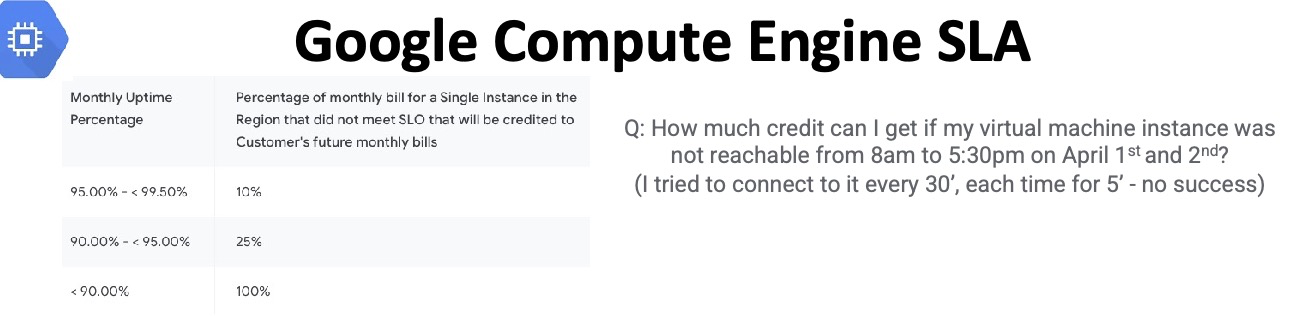
\includegraphics[width=0.7\textwidth]{1.png}
    \caption{Google rimborsa (sotto forma di credito) "fino al 100\%" delle spese in caso di downtime}
\end{figure}

\subsubsection{Uptime}
\begin{definition}[Monthly Uptime Percentage]
    $$\text{MPU = } \frac{\text{\# minuti in un mese - \# minuti di downtime}}{\text{\# minuti in un mese}}$$
\end{definition}

\newpage
\subsubsection{Downtime}
\begin{definition}[Downtime Period]
    \textbf{Minuti consecutivi} di downtime
\end{definition}
\paragraph{Come Google conteggia il downtime} I minuti parziali (e.g. 2m 30s) sono arrotondati per difetto (2m 30s $\rightarrow$ 2m), mentre qualsiasi downtime per un intervallo di tempo inferiore a 1 minuto non viene neanche considerato da Google.\\
Ma quindi quanto credito posso riavere indietro, nel caso in cui per due giorni di fila il servizio è down dalle 8 alle 17:30 e io provo a connettermi senza successo ogni 30 minuti, insistendo ogni volta per 5 minuti?\\
Risposta: il Monthly Uptime Percentage è $$ \text{MUP} = \frac{(30\cdot 24\cdot 60)-(2\cdot 20\cdot 5)}{30\cdot 24\cdot 60} = \frac{43000}{43200} = 0.955$$ quindi non rientro neanche nella soglia per il 10\%

\subsection{Errori comuni nell'adozione del Cloud}
\paragraph{Overprovisioning e Underprovisioning}
Quando si realizza un servizio è difficile predire quanto crescerà la domanda nel tempo e di conseguenza la quantità di risorse che saranno necessarie. In tal senso si parla di overprovisioning e underprovisioning.
\begin{definition}[Overprovisioning]
gestire in anticipo un eventuale flusso di utenti in crescita. Utilizzo overkill (eccessivo) di risorse rispetto a quelle effettivamente necessarie con conseguente spreco di risorse    
\end{definition}

\begin{definition}[Underprovisioning]
se il picco di utenti è sottostimato, il servizio risulterà in una cattiva user experience e gli utenti che non riescono ad accedere al servizio difficilmente ritorneranno
\end{definition}

\subsection{Vantaggi (alcuni) del Cloud}
Con il Cloud non serve fare previsione sulle richieste perché le risorse appaiono ”illimitate” agli occhi dell'utente e soprattutto disponibili on-demand. Il nome Cloud deriva dal fatto che quando si disegnava lo schema client-server, tutto ciò che stava fra i due veniva rappresentato come una nuvoletta per semplicità.\\
Dal punto di vista \textbf{economico}:
\begin{itemize}
    \item non servono un investimento e una progettazione iniziale per l’infrastruttura hardware, infatti si possono realizzare e offrire servizi hostati interamente sul Cloud
    \item servizi \textbf{pay-per-use}: paghi solamente ciò che usi, tipicamente vengono preferiti anche se si va a spendere di più perché garantiscono \textbf{elasticità} e permettono di \textbf{trasferire il rischio su terzi} cioè se qualcosa va storto il responsabile è il provider del servizio Cloud
    \item Il modello di business introdotto dal Cloud Computing permette di trasformare alcuni costi fissi in \textbf{costi variabili} e permette uno shift da spese CapEx a spese \textbf{OpEx}
\end{itemize}

\subsection{Modelli di servizio}
\paragraph{Infrastucture as a Service (IaaS)} fornisce server, memoria, rete (virtualizzati), il fornitore di servizi IaaS gestisce tutta l’infrastruttura. Il cliente è responsabile di tutti gli altri aspetti del deployment (per esempio sistema operativo, applicazione). Il mercato del Cloud IAAS è cresciuto del 31.3\% nel 2018. Esempi di IaaS sono \textbf{Amazon EC2} (instances) e \textbf{Amazon S3} (buckets)
\paragraph{Platform as a Service (PaaS)} fornisce un’intera piattaforma come un servizio (macchine virtuali, sistema operativo, servizi, ambiente di sviluppo), quindi il fornitore PaaS gestisce infrastruttura + sistema operativo + enabling software. Il cliente è responsabile di installare e gestire l’applicazione. Esempi di PaaS sono: Heroku, Azure, Google App Engine
\paragraph{Software as a Service (SaaS)} fornisce software on-demand accessibile mediante client thin o API, quindi il fornitore SaaS gestisce l’infrastruttura + sistema operativo + applicazione e il cliente non è responsabile di niente.  Esempi: Salesforce.com, Google Drive
La differenza tra IaaS e PaaS è lieve, se offri PaaS spesso sei obbligato a offrire anche IaaS

\newpage
\subsection{Modelli di deployment}
\paragraph{Pubblico}il vantaggio è la scalabilità, però l'utente ha poco controllo su come sono gestiti i dati (ad esempio se succede qualcosa nei datacenter di Amazon, i nostri dati sono violati)
\paragraph{Privato} non ha molta scalabilità però c'è più sicurezza di dati
\paragraph{Ibrido} soluzione molto utilizzata, si tengono sul cloud privato i dati sui quali si vuole avere pieno controllo e privacy, i restanti su un cloud pubblico fornito da un cloud provider

\begin{figure}[h!]
    \centering
    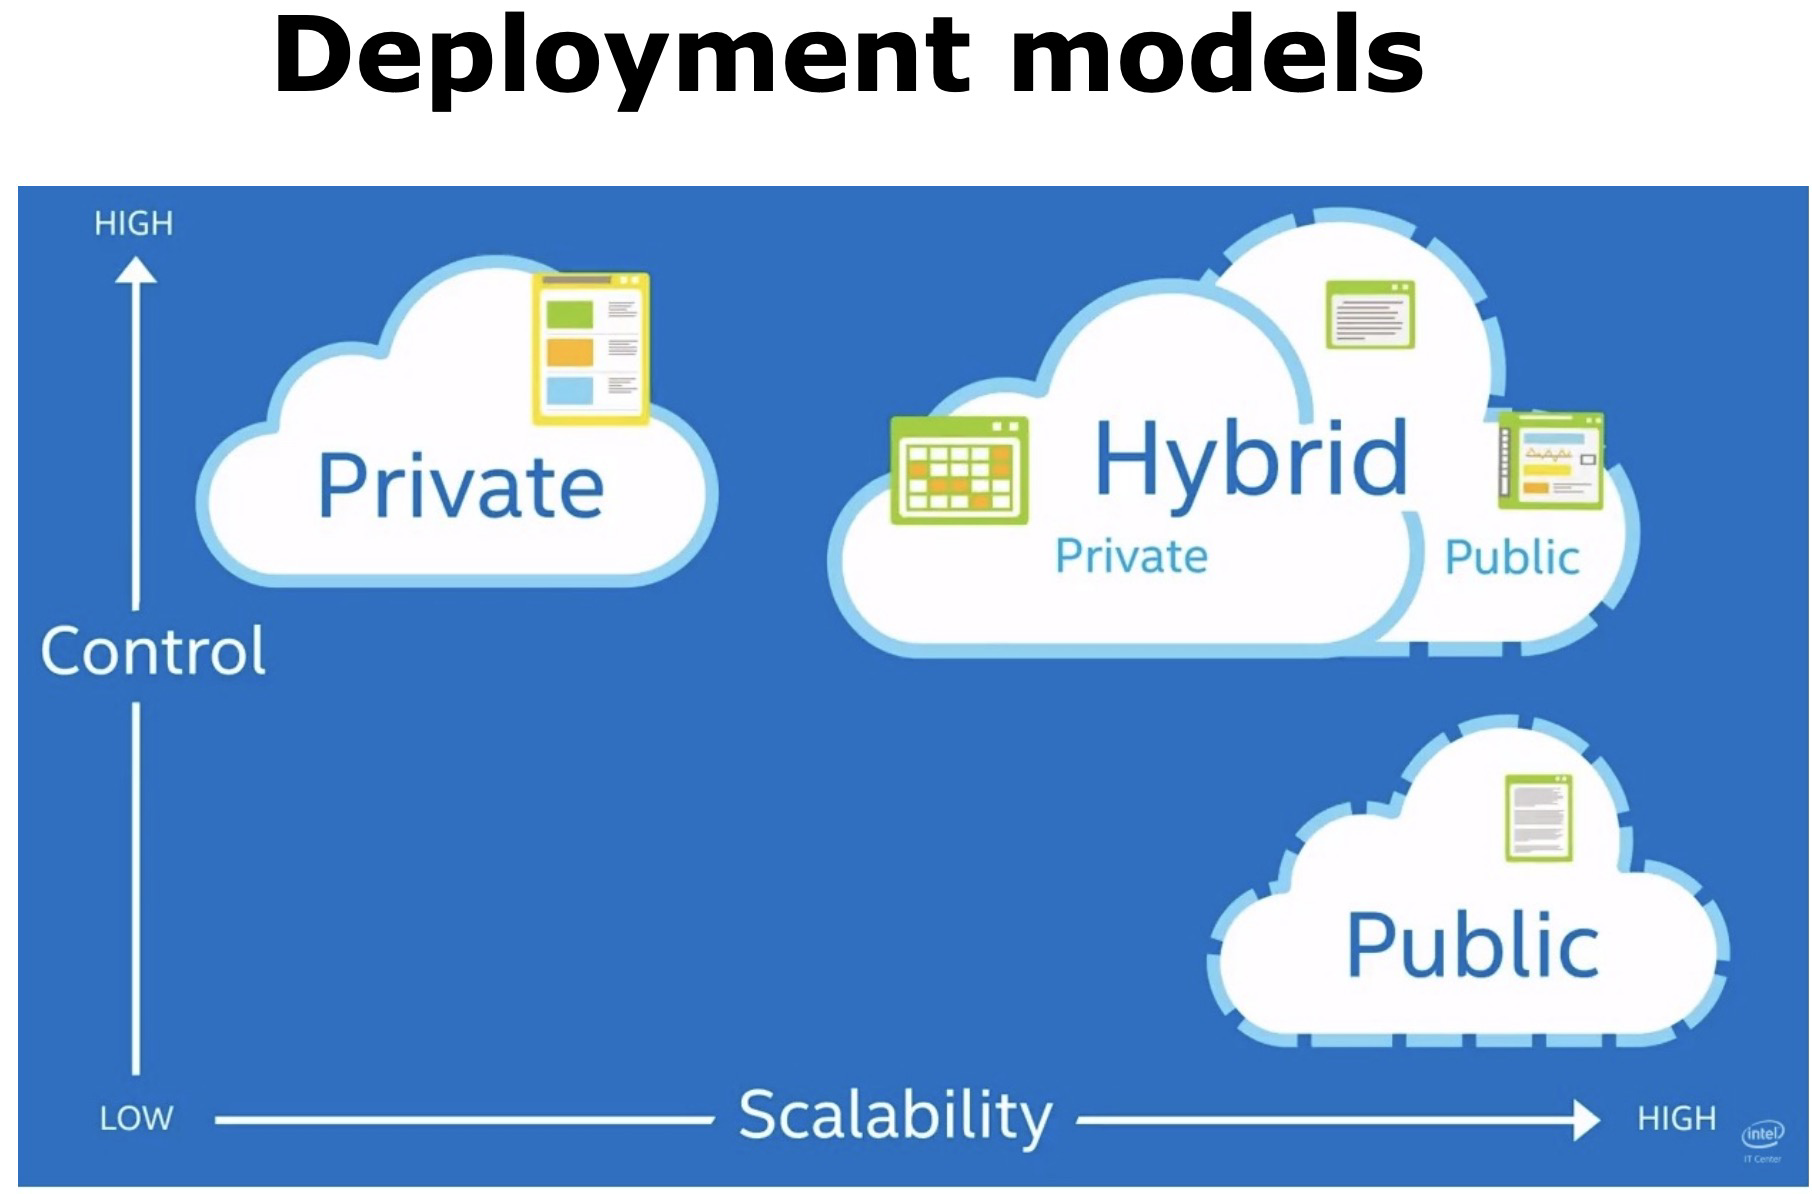
\includegraphics[width=0.7\textwidth]{2.png}
    \caption{trade-off da considerare per i vari tipi di deployment}
    %\label{fig:enter-label}
\end{figure}

\subsection{Ostacoli per l'adozione del Cloud}
\begin{itemize}
    \item \textbf{Confidenzialità dei dati}: dove verranno memorizzati i nostri dati concretamente? Privacy e integrità dei dati sono garantiti? Come? Come si può sapere se si è verificato un problema?
    \item \textbf{Disponibilità dei servizi}: cosa succede se un Cloud provider fallisce? Spesso le aziende si affidano ad un solo Cloud provider ma bisogna usarne di più (no \textit{single point of failure}, il sistema deve essere fault tolerant). Bisogna anche mettere in conto che ci saranno dei fallimenti temporanei e il servizio potrebbe non essere disponibile in alcuni momenti
    \item \textbf{Vendor lock-in}: più vengono utilizzate funzioni del Cloud più si rimane ”incatenati” all'ecosistema di quel provider perché se proviamo a spostare i nostri dati altrove dovremmo modificare tutte le nostre applicazioni per portarle su altri Cloud. Si tratta di un lock-in tecnologico legato alla difficoltà nella transizione verso un altro provider, non c'è nessuna clausola contrattuale che impedisce di abbandonare l'ecosistema del provider
\end{itemize}
\newpage
\section{IaaS (Infrastructure as a Service)}
\subsection{Virtualization}
\paragraph{Virtualizzazione} con questo termine si intende la creazione di risorse virtuali come server, spazio di archiviazione o network. Serve per gestire il carico di lavoro rendendo la computazione più \textbf{scalabile}. La forma più comune di virtualizzazione è il \textbf{Server}.\\
La virtualizzazione è un livello di \textbf{astrazione}: il SO è astratto dall'hardware e non è più legato al server/pc dove gira.

\subsubsection{Server Virtualization} Con Server Virtualization si intende il livello di virtualizzazione tra il server fisico e il sistema operativo. Comprende le macchine virtuali sulle quali viene installato il sistema operativo e le applicazioni. Così come il SO permette a tutti i programmi e software di funzionare, il livello di virtualizzazione permette di avere tante macchine virtuali.
\begin{itemize}
    \item \textbf{Virtual Host}: server fisico su cui girano le altre VM
    \item \textbf{Virtual Machine}: ogni SO ospite del Virtual Host
\end{itemize}

\subsubsection{Hypervisor} L'hypervisor è una funzione che crea il livello di virtualizzazione (o \textit{virtualization layer}, permette la virtualizzazione del server) e contiene il Virtual Machine Manager (VMM) per la gestione delle VM.
Il sistema operativo non è installato direttamente sulla macchina ma è astratto dall’hardware: esiste un livello di astrazione tra il server e il sistema operativo chiamato \textbf{virtualization layer} (per esempio ESXi o ESX di VMWare). 
Al livello sopra il virtualization layer ci sono le macchine virtuali, sulle quali è possibile installare un SO.
Esempi di hypervisor: \textit{Vmware Workstation, Virtual Server, Hyper-V , Fusion, XenServer}

\paragraph{Tipi di Hypervisor}
\begin{itemize}
    \item \textbf{Tipo 1}: installato direttamente sull’hardware, e.g. Hyper-V, ESX, ESXi, XenServer
    \item \textbf{Tipo 2}: installato sull’OS dell’hardware come una normale applicazione, e.g. Workstation, Virtual Server, Fusion, Oracle VirtualBox
\end{itemize}
Il tipo 1 è più performante, il tipo 2 non riesce a mantenere più VM contemporaneamente però è più adatto per hardware meno potenti ad esempio un laptop

\subsection{Amazon}
\textbf{Amazon}, fondata inizialmente con il nome di “Cadabra” nel 1994 da Jeff Bezos, era una biblioteca online. Il business plan iniziale era di non aspettarsi profitto per i primi 4-5 anni, il primo profitto lo hanno avuto nel 2001.\\
Ad oggi Amazon detiene quasi il 50\% del mercato Cloud, più precisamente il 47.8\% (seguito da Microsoft 15\%, Alibaba 7\%, Google 4\%). Alcuni dati:
\begin{itemize}
    \item 300 milioni di utenti (Dicembre 2017)
    \item 2 milioni di venditori Amazon (Gennaio 2018)
    \item 560.000 dipendenti (Gennaio 2018)
    \item 3.724 miliardi di dollari di entrate all’anno
\end{itemize}

\subsubsection{Amazon Elastic Compute Cloud (EC2)}
È difficile prevedere il numero di server di cui abbiamo bisogno per un'applicazione, per questo Amazon EC2 mette a disposizione dei server virtuali chiamati \textbf{istanze} configurabili (ad esempio con la scelta di un template Windows/Linux). Si può scegliere tramite Amazon Web Services (\textbf{AWS}) management console (o librerie SDK) la potenza di calcolo delle istanze in base alle proprie necessità. Le istanze si possono scegliere in base a CPU, memoria, storage e GPU.\\
Amazon EC2 ci offre anche un buon livello di sicurezza grazie al \href{https://aws.amazon.com/it/vpc/}{VPC} (Virtual Private Cloud) che rende la connessione più sicura all’interno del Cloud.\\
Inoltre esiste Amazon Elastic Block Store (\textbf{EBS}) che garantisce uno \textbf{storage persistente} per l’uso su EC2, offrendo disponibilità e durabilità dei nostri dati. È stato pensato per le applicazioni che necessitano di big data analytics, stream processing o data warehouse.\\
\textbf{Autoscaling}: Amazon permette di definire delle metriche per decidere come e quando “scalare”, e farlo automaticamente all’occorrenza\\
Per quanto riguarda i \textbf{prezzi}:
\begin{itemize}
    \item \textbf{On demand}: paghi solo per quello che utilizzi (ad esempio prezzo per GB)
    \item \textbf{Reserved instances}: pagamento mensile (cheaper than on-demand), si usa quando si sa già a priori quali e quante macchine serviranno
    \item \textbf{Spot Instances}: sono istanze inutilizzate che Amazon mette in vendita ogni 5 minuti all’asta (fino al 90\% più economiche di quelle on-demand, tipicamente intorno al 50\%)
    \item \textbf{Dedicated hosts}: server fisico con istanze EC2 totalmente dedicato all'utente
    \item \textbf{AWS Free Tier}: livello freemium con limitazioni
\end{itemize}

\subsubsection{Amazon Simple Storage Server (S3)}
Al fine di gestire l’archiviazione dei dati della propria applicazione, Amazon S3 mette a disposizione un servizio di \textbf{storage}. L’interfaccia è estremamente semplice: \textit{drag and drop} in un secchiello (\textbf{bucket}).\\
Amazon S3, per far fronte ad eventuali perdite di dati, esegue 3 backup su 3 unità di memoria diverse e consente di mantenere tutte le vecchie versioni dei file in modo da poterli recuperare se cancellati erroneamente.
Anche per S3 si paga solo quello che si utilizza (\textit{pay per use}).\\
Ci sono diverse  classi di memorizzazione:
\begin{itemize}
    \item \textbf{s3 standard}: oggetti comuni con lettura continua (\$0.023/ GB)
    \item s3 standard \textbf{infrequent access}: accesso poco frequente a questi dati (\$0.012/ GB)
    \item \textbf{Amazon Glacier} per dati da memorizzare a lungo termine, e.g. backup di un database (\$0.004/ GB)
\end{itemize}
Per quanto riguarda i prezzi, si paga per GB e in base alla classe di memorizzazione, ma anche qui si ha un AWS Free Usage Tier con 5GB gratuiti.

\subsection{Dropbox}
Dropbox è stato fondato nel 2007 con l'idea di offrire gratuitamente spazio di archiviazione con limitazioni, con l'opzione di passare al piano premium per avere più storage. A Marzo 2016 Dropbox aveva 500 milioni di utenti.\\
Per i primi 8 anni Dropbox ha sempre usato i server di Amazon S3, (metadati sulle proprie macchine, files su S3) ed era il loro più grande cliente, poi tra il 2014 il 2016 ha costruito le proprie macchine per avere il pieno controllo sui dati. Tuttavia, al momento del passaggio da Amazon S3 ai propri server hanno avuto molti problemi:
\begin{enumerate}
    \item trasferire tutto prima del rinnovo del contratto con Amazon
    \item gli utenti non si sarebbero dovuti accorgere di niente, non avrebbero dovuto avere interruzioni di servizio o perdite di dati nonostante ci volesse 1 giorno intero per trasferire 4 petabyte.
    \item il nuovo software \textit{Magic Pocket} non era totalmente compatibile con il nuovo hardware, hanno dovuto fare delle modifiche rinominandolo \textit{Mozilla Rust}
    \item incidenti stradali per i camion che trasportavano i server hardware
\end{enumerate}

\begin{figure}[h!]
    \centering
    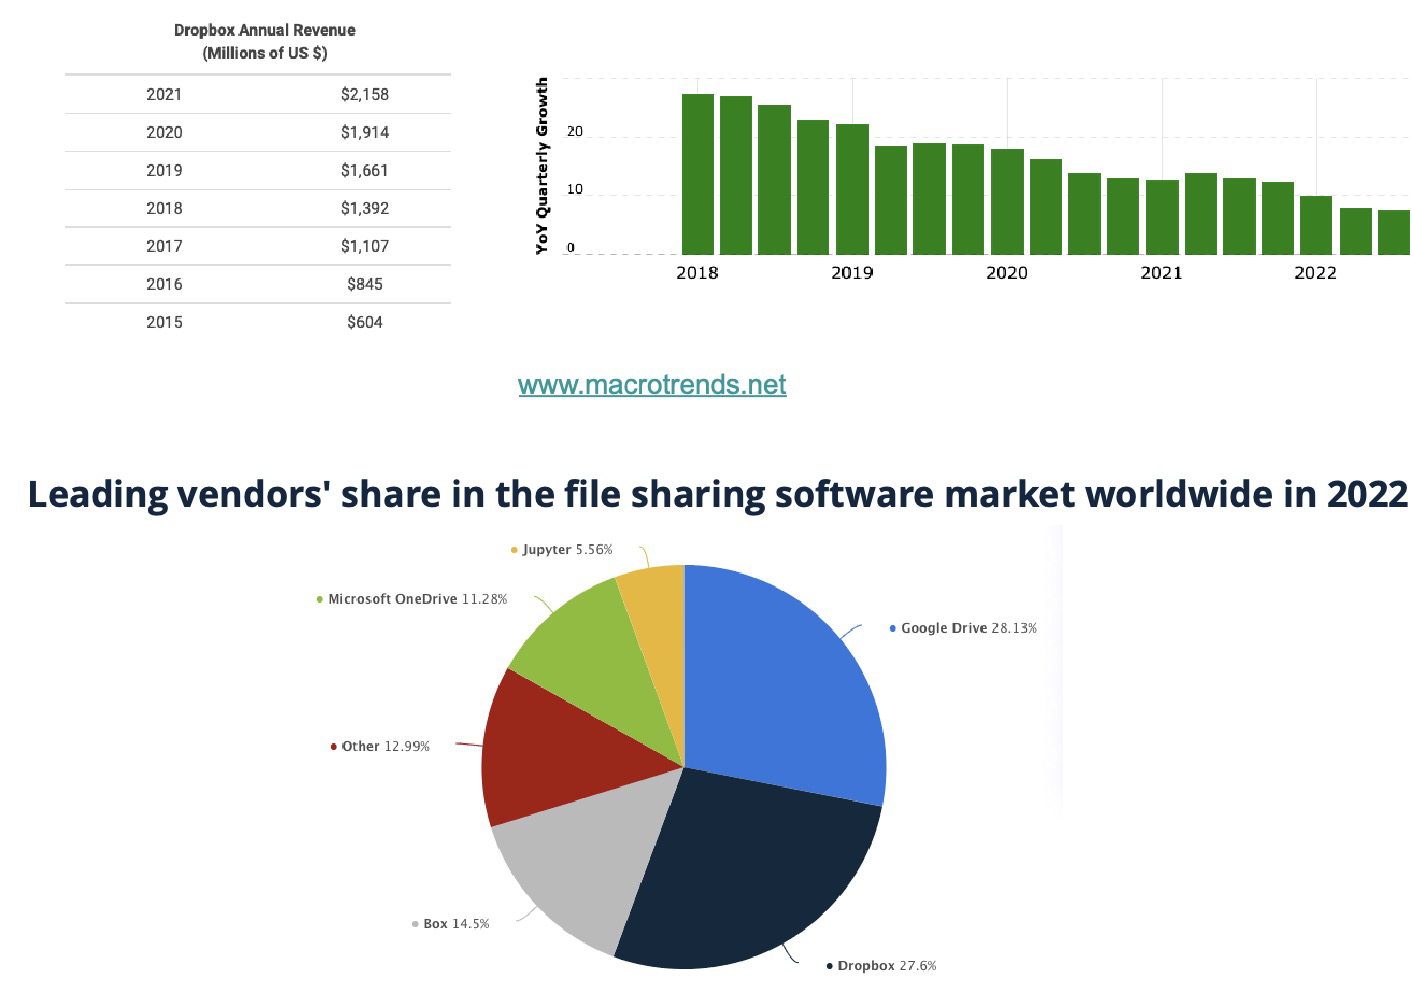
\includegraphics[width=0.7\textwidth]{3.png}
    \caption{Shares del mercato Cloud (2019)}
    %\label{fig:enter-label}
\end{figure}

\paragraph{SLA di Dropbox vs Amazon}
\href{https://aws.amazon.com/agreement}{SLA di AWS} : cosa ci garantisce Amazon? \textbf{Niente}. \textit{The service Offering Are Provided “As is”}.\\
Amazon non dà garanzia riguardo ai servizi offerti, garanzia contrattuale pari a zero.\\
Analogamente il SLA di Dropbox, che non garantisce nessun diritto se ci sono perdite di business, profitto o dati.

\newpage
\paragraph{Come suddividere un’applicazione three-tier su un Cloud ibrido?} 
\begin{enumerate}
    \item Web server (presentation tier)
    \item App server (business logic tier)
    \item DB server (data tier)
\end{enumerate}
In generale qualsiasi soluzione va bene, solitamente si mettono almeno 2 parti sul Cloud pubblico, in alcuni casi anche tutto. Più raramente viene usato solo il Cloud privato.

\subsection{AWS IAM}
AWS IAM  (\textbf{I}dentity and \textbf{A}ccess \textbf{M}anagement) permette di controllare e gestire l'accesso degli utenti ai servizi AWS. IAM consente di creare utenti, gruppi di utenti e policy di autorizzazione per controllare quale operazione può essere eseguita da ogni utente o gruppo. In questo modo è garantito che solo utenti autorizzati possano accedere e gestire determinate risorse.\\
In particolare, IAM permette di:
\begin{itemize}
    \item gesitre gli utenti di IAM e i loro accessi
    \item gestire ruoli e permessi
    \item autenticazione federata: accedere autenticandosi tramite Google
\end{itemize}

\paragraph{Access management} che cosa ha diritto di fare un utente dopo che si è autenticato, e.g. quali dati può vedere e quali può modificare
L' autenticazione  ad IAM si può effettuare tramite la GUI della dashboard, tramite CLI di AWS o tramite kit di development (SDK)
\begin{figure}[h!]
    \centering
    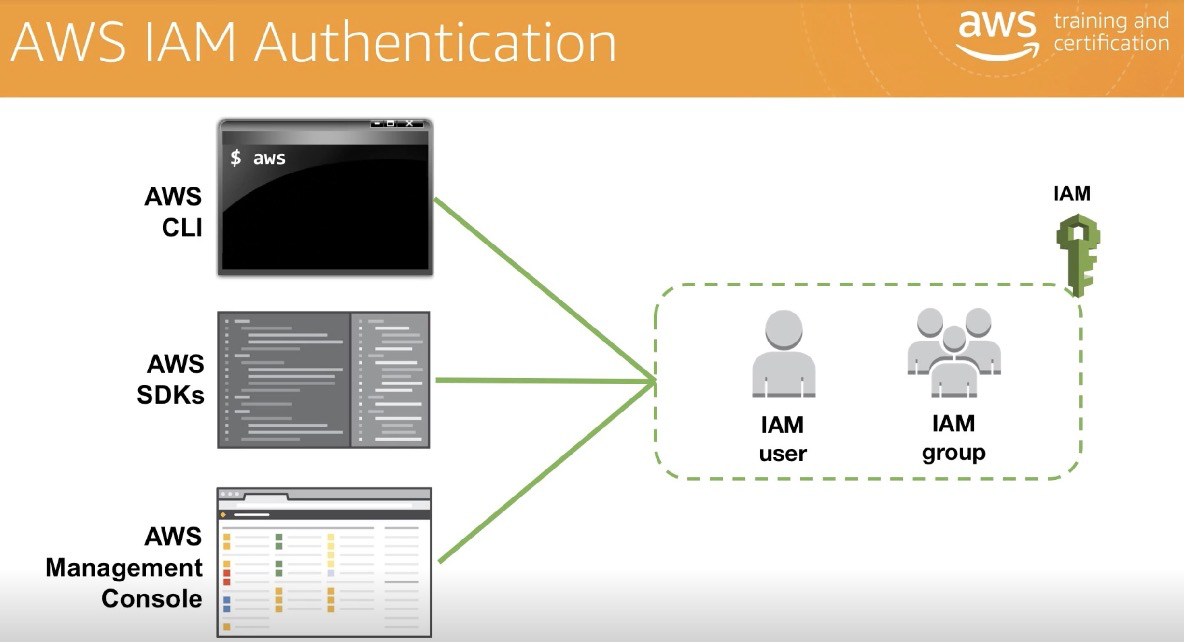
\includegraphics[width=0.6\textwidth]{4.png}
    \caption{Possibili metodi di autenticazione con AWS IAM}
    \label{fig:enter-label}
\end{figure}
\newpage
I  permessi  di IAM sono definiti tramite  \textbf{policy} , che non sono altro dei file \textbf{JSON} in cui sono salvati i permessi degli utenti. Uno use-case è ad esempio quando si crea un bucket si può associare una policy di pieno accesso/read only alle risorse
\begin{figure}[h!]
    \centering
    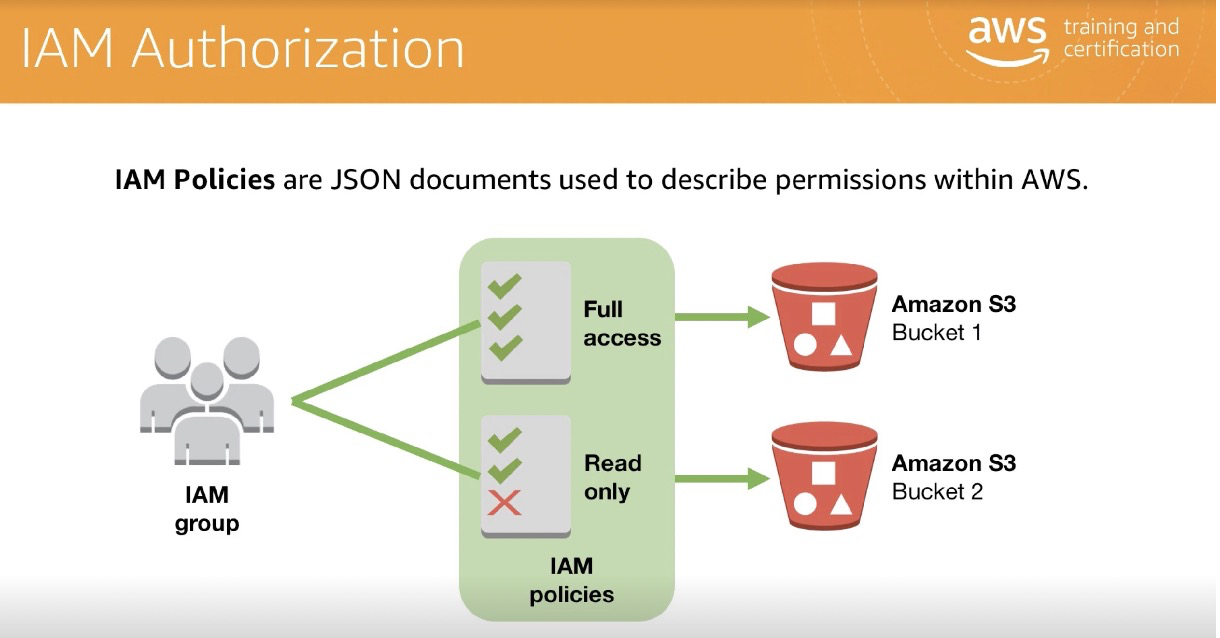
\includegraphics[width=0.6\textwidth]{5.png}
    \caption{IAM group}
    \label{fig:enter-label}
\end{figure}

Infine, IAM permette anche di creare gruppi di utenti e utenti individuali e assegnare dei ruoli a determinati gruppi/individui
\begin{figure}[h!]
    \centering
    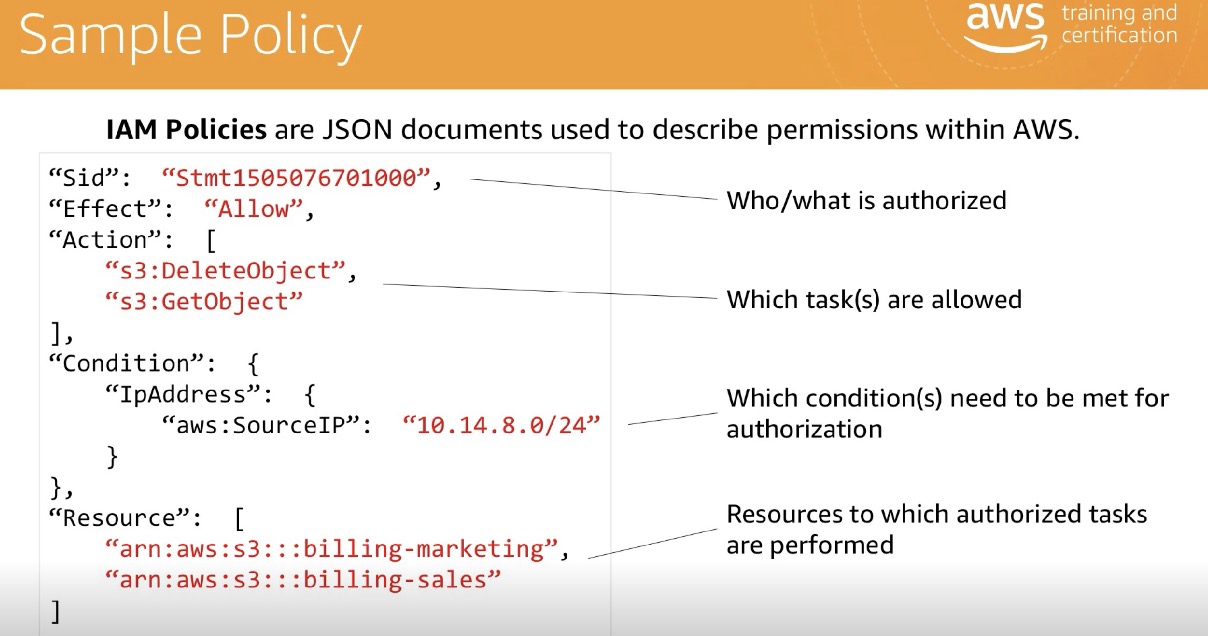
\includegraphics[width=0.6\textwidth]{6.png}
    \caption{IAM Policies, file JSON per gestire i permessi e l'accesso alle risorse}
    \label{fig:enter-label}
\end{figure}
\newpage
\section{Laboratorio: AWS} \label{lab1}

Hands-on sulle seguenti funzionalità offerte da AWS
\begin{itemize}
    \item \textbf{Storage}: Amazon Simple Storage Service (\textbf{S3})
    \item \textbf{Calcolo}: Amazon Elastic Compute Cloud (\textbf{EC2})
    \item \textbf{Sicurezza}: AWS Identity and Access Management (\textbf{IAM})
\end{itemize}

\subsection{Svolgimento}
\begin{enumerate}
    \item Creare un \textbf{bucket} su S3
    
    \item Creare una coppia di chiavi (\textbf{key pair}) su EC2, key pair scaricato come file con estensione \textit{.pem}
    
    \item Creare un'\textbf{istanza EC2} selezionando la coppia di chiavi creata nello step precedente. Per l'istanza abbiamo usato il SO Amazon Linux 2 e \textit{t2.micro} per rispettare il free plan
    
    \item Accedere da terminale:
    \begin{enumerate}
        \item aprire un terminale nella directory contenente il file \textit{keypair.pem} e inviare il comando \verb|chmod 400 keypair.pem|
        \item accedere tramite \textbf{SSH} all'istanza EC2: \verb|ssh –i keypair.pem ec2-user@<IPv4_DELLA_MIA_ISTANZA>|
    \end{enumerate}

    \item Caricare e gestire file tra S3 e EC2 tramite la CLI di AWS:
    \begin{enumerate}
        \item caricare un file sul bucket S3
        \item scaricare il file tramite il terminale dell'istanza con il comando: \verb|aws s3 mv s3://<BUCKET>/<FILE> <LOCAL_PATH>|
        \begin{itemize}
            \item Il comando non funziona perché non ho ancora i permessi, infatti per accedere al bucket S3 dalle istanze EC2 è necessario creare un Ruolo IAM per concedere l’accesso
        \end{itemize}
    \end{enumerate}

    \item Creare un \textbf{IAM Role}: in questo caso abbiamo garantito accesso completo (\textit{AmazonS3FullAccess})

    \item Aggiungere il Ruolo IAM all’istanza EC2 e riprovare il comando precedente
    
\end{enumerate}

\subsection{Caricare un file su S3 da EC2}
Partendo da un file in locale, caricarlo tramite SSH nell'istanza poi tramite terminale caricare il file dall'istanza al bucket S3
\begin{lstlisting}[language=bash]
    scp -i chiavi.pem <FILE> ec2-user@<IPv4_EC2_INST>:<REMOTE_PATH>
    aws s3 mv <FILE> s3://<BUCKET>
\end{lstlisting}

\subsection{Bash script per sorting su EC2}
Scrivere uno script bash che svolga le seguenti funzioni:
\begin{enumerate}
    \item Scarica un file dal bucket S3. Il file è formato da una lista non ordinata di interi, uno per riga
    \item Li ordina
    \item Carica la lista ordinata su S3
\end{enumerate}
Codice:
\begin{lstlisting}[language=bash]
    aws s3 mv s3://<BUCKET>/numbers.txt ./numbers.txt
    sort -n -o numbers.txt numbers.txt
    aws s3 mv ./numbers.txt s3://<BUCKET>/numbers.txt    
\end{lstlisting}

\paragraph{Approfondimento} installare un Web Server Apache su un'istanza EC2. \href{https://cloudkatha.com/how-to-install-apache-web-server- on-amazon-linux-2/}{Guida}
\newpage
\section{Containers} \label{container}
\subsection{Differenze tra VM e Container}
Sia nelle macchine virtuali e Container vi è un livello di \textbf{virtualizzazione} (hypervisor e docker engine) ma nei Container manca il sistema operativo guest e il container manager sostituisce l'hypervisor. Inoltre i Container hanno altri vantaggi:
\begin{itemize}
    \item Sono più leggeri, ovvero un Container chiede ad un server meno risorse rispetto ad una macchina virtuale
    \item I tempi di avvio sono molto più brevi rispetto ad una macchina virtuale
    \item Sono più semplici da costruire rispetto ad una macchina virtuale
\end{itemize}
Tuttavia, i Container condividono più risorse all’interno di un server fisico e questo implica che c’è meno isolamento rispetto ad una macchina virtuale, e quindi c’è una superficie più ampia per attacchi di sicurezza. In altre parole un Container è meno sicuro rispetto ad una macchina virtuale.
\begin{figure}[h!]
    \centering
    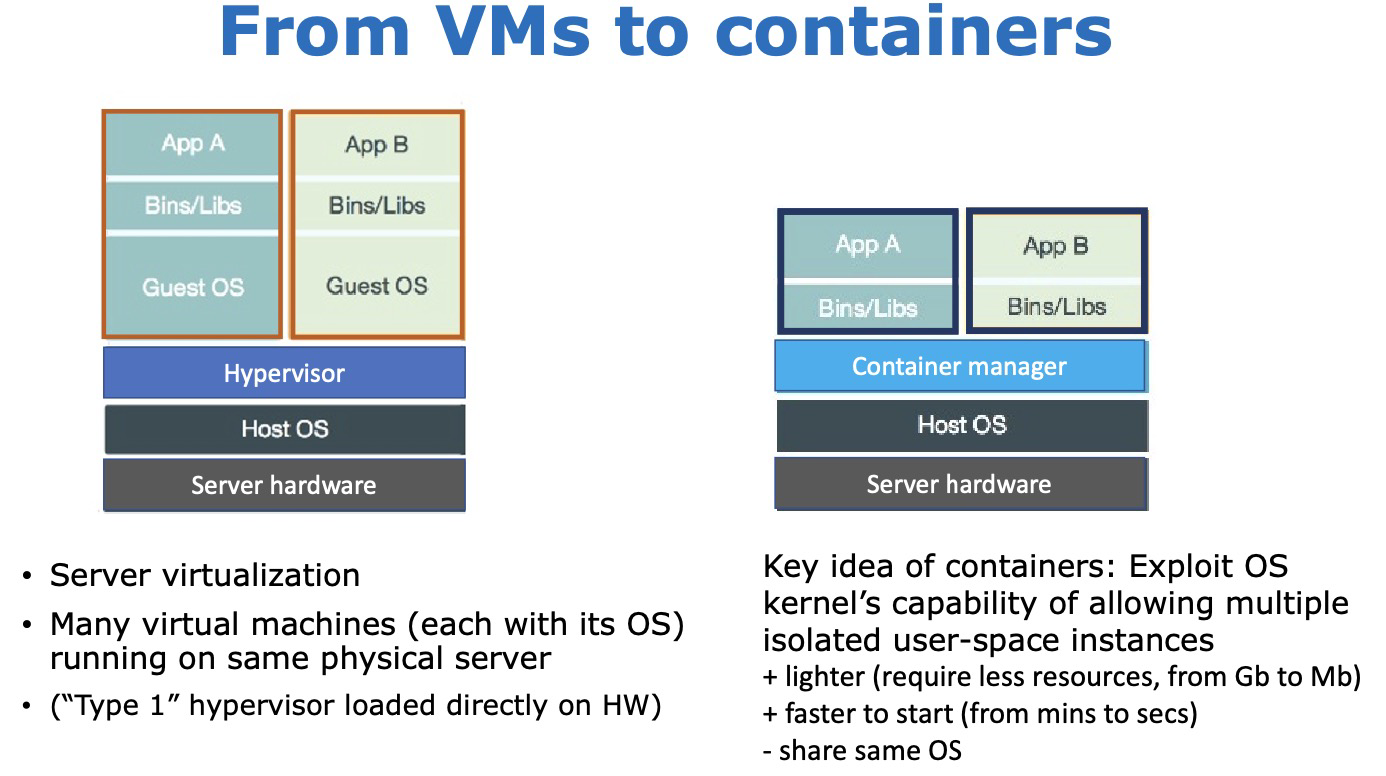
\includegraphics[width=0.5\textwidth]{7.png}
    \caption{VM e Container}
    \label{fig:enter-label}
\end{figure}

\subsection{Docker}
\paragraph{Storia di Docker} I container non sono un'idea molto recente, infatti il sistema operativo UNIX forniva un comando \verb|chroot| che permetteva una forma di isolamento del filesystem.\\
La prima soluzione completa basata su Container fu LXC di Linux Container nel 2008. Nel 2013 il fenomeno è ”esploso” con Docker, che ha aggiunto la portabilità delle immagini e un'interfaccia user-friendly.\\
Docker offre un \textbf{docker engine} per la creazione ed esecuzione di Container e \textbf{docker hub} per pubblicare e scaricare immagini di Container

\paragraph{Come funziona} Docker è una piattaforma che consente di eseguire applicazioni in ambiente isolato, dando la possibilità di sviluppare ed eseguire applicazioni \textbf{portabili} grazie ai containers.\\
In pratica, Docker sfrutta la virtualizzazione basata sui container per eseguire più istanze isolate sullo stesso sistema operativo.
I Container sono \textbf{volatili} ovvero non tengono traccia dei dati una volta terminata l’esecuzione. Per garantire che i dati siano persistenti esistono  i \textbf{volumi}.\\
L’applicazione viene impacchettata in una \textbf{immagine} ovvero un file read-only che rappresenta l’intera applicazione e che permette di mandare in esecuzione un Container. I template (immagini) vengono memorizzati in un \textbf{registry} (per esempio Docker registry) che è strutturato in repositories. Ogni repository contiene un insieme di immagini per versioni diverse del software.\\
Le immagini vengono identificate dalle coppie \textit{repository:tag} e sono \textbf{stratificabili}, cioè strutturate in livelli (layers): al livello più basso vi è il \textit{base image}.\\
Il Container andrà in esecuzione in cima a questa pila di layers e a seconda del tipo di applicazione può effettuare delle modifiche che possono a loro volta essere committate in una nuova immagine.\\

\newpage
\paragraph{Commands} I comandi principali da conoscere per Docker sono:
\begin{itemize}
    \item \verb|pull| scarica un’immagine da un Docker registry
    \item \verb|run| manda in esecuzione il Container definito dall’immagine
    \item \verb|commit| per creare ed effettuare delle modifiche, committate in una nuova immagine
    \item \verb|build| per costruire l'immagine partendo da un \textbf{Dockerfile}, che funziona come una sorta di Makefile
\end{itemize}

\begin{figure}[h!]
    \centering
    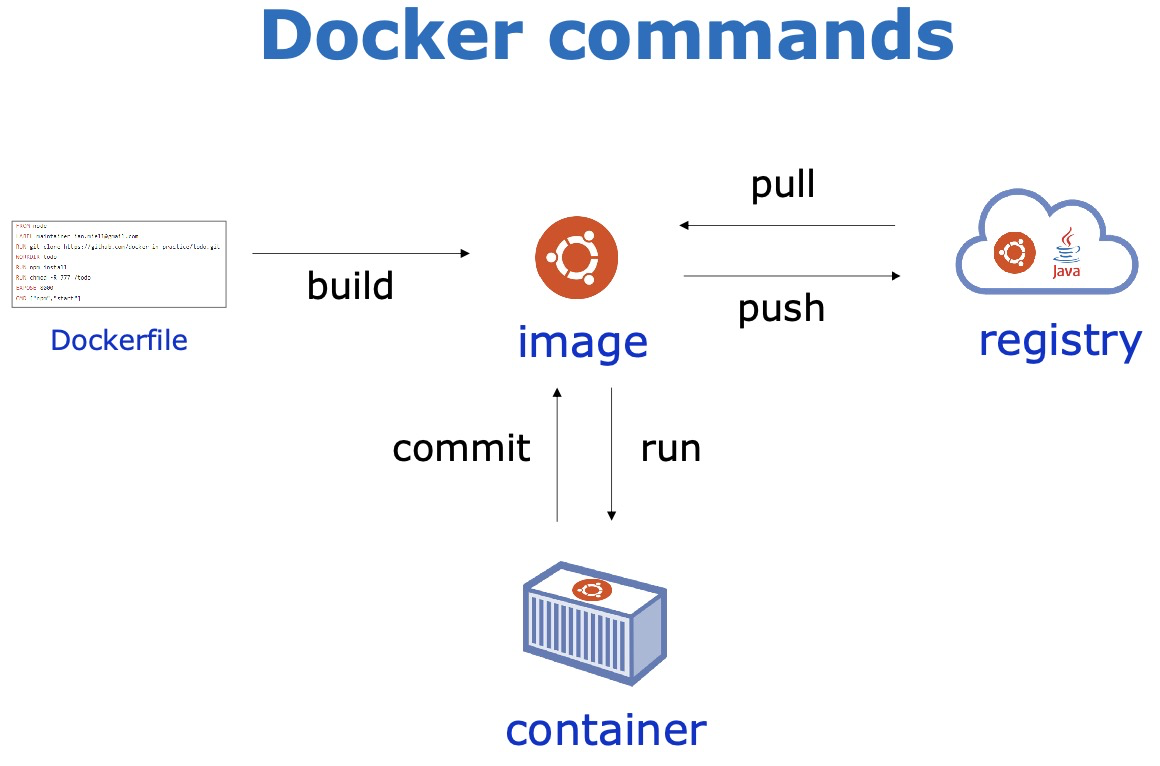
\includegraphics[width=0.7\textwidth]{8.png}
    \caption{Comandi principali di Docker}
    \label{fig:enter-label}
\end{figure}

\paragraph{Demo (DIY)} In \href{https://www.youtube.com/watch?v=YFl2mCHdv24}{questa demo} viene usato un volume per aggiornare la pagina web real time (come già detto, con i volumi i dati sono persistenti)
Il \verb|docker-compose| permette di specificare come si vuole che sia formata l’applicazione multiservizio da mandare in esecuzione.\\
\href{https://www.youtube.com/watch?v=Qw9zlE3t8Ko}{Docker Compose video visto in aula}

\begin{figure}[h!]
    \centering
    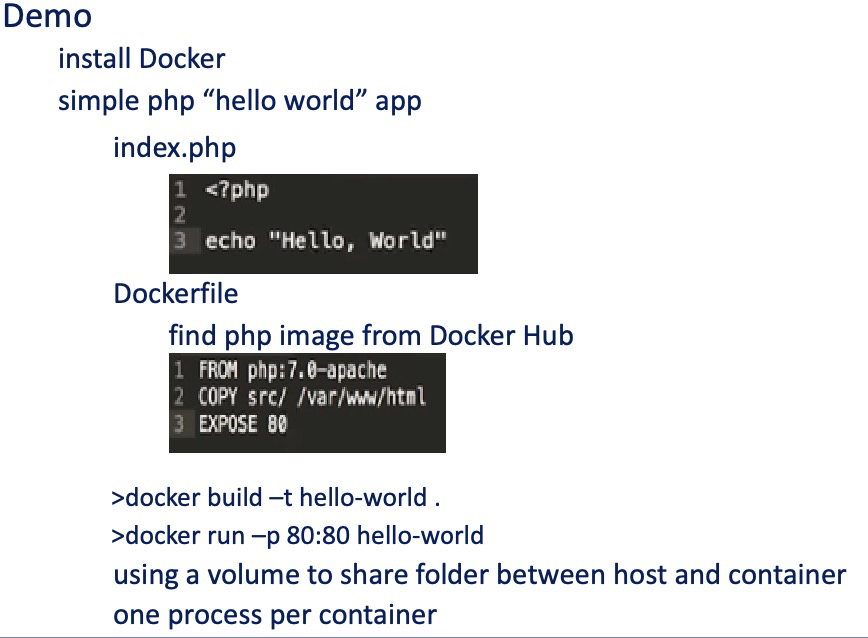
\includegraphics[width=0.5\textwidth]{9.png}
    \caption{Docker demo}
    %\label{fig:enter-label}
\end{figure}

\paragraph{Docker Swarm} Un’altra feature di Docker è la \textbf{swarm mode}, un approccio dichiarativo (l'utente dichiara l'organizzazione che desidera ottenere) che permette di gestire un insieme (cluster) di host Docker chiamati \textit{swarm}.\\
Quindi i vari task vengono ripartiti tra host diversi. I nodi del cluster possono avere due ruoli:
\begin{itemize}
    \item \textit{manager}, che delegano e distribuiscono i task ai workers
    \item \textit{workers}, che eseguono i task
\end{itemize}
L’utente può definire lo stato per la configurazione a tempo di esecuzione dell’applicazione. Gli swarm manager effettuano un \textbf{monitoraggio costante} delle attività e interviene qualora vi sia una differenza tra lo stato attuale e lo stato desiderato dall’utente.\\
Per esempio se l’utente desidera che vi siano in esecuzione 10 repliche dello stesso container, il manager swarm distribuisce le 10 repliche sulle macchine workers; se una worker machine ospita due repliche e si blocca, il manager swarm crea due nuove repliche che vengono assegnate ad altre worker machine disponibili ed in esecuzione
\begin{figure}[h!]
    \centering
    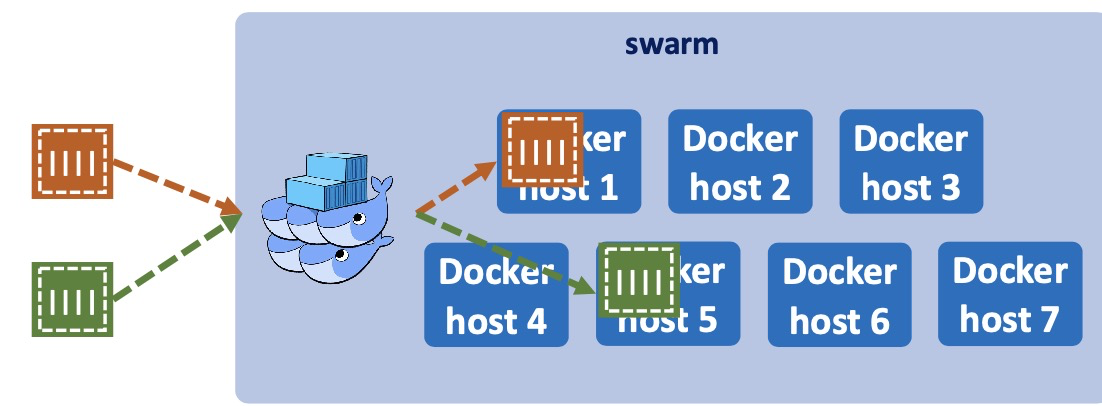
\includegraphics[width=0.7\textwidth]{10.png}
    \caption{Docker swarm}
    %\label{fig:enter-label}
\end{figure}

\subsection{Kubernetes}
Nel 2014, dopo il successo di Docker, è stato lanciato Kubernetes che è un sistema per l'orchestrazione di Container. Kubernetes possiede molte funzionalità simili a Docker swarm ma è più efficiente. Docker e Kubernetes non sono in contrapposizione tra di loro, ma si integrano a vicenda.\\
Un \textbf{pod} è un gruppo di uno o più Containers con storage/rete condivisa, e con una specifica per come gestire i Container. I contenuti del pod vengono allocati e schedulati per essere eseguite in contesto condiviso.\\
Un \textbf{kubelet} è un \textit{node agent} che è in esecuzione \textbf{su ogni nodo} che prende un insieme di specifiche pod (principalmente attraverso il server API) e assicura che i Container descritti in tali specifiche siano in esecuzione e ”sani”.\\
\href{https://www.youtube.com/watch?v=PH-2FfFD2PU}{Video su Kubernetes visto in aula}

\paragraph{Docker Swarm vs Kubernetes} Così come docker swarm, anche kubernetes serve per l'orchestrazione di containers. La differenza sta nella semplicità e nella potenza: Swarm è più semplice da installare ed è abbastanza semplice da imparare. Kubernetes offre il meccanismo di \textbf{auto-scaling}, è più robusto in termini di tolleranza ai guasti.\\
Quindi se l’applicazione che si deve gestire è relativamente semplice, Docker Swarm probabilmente è la scelta giusta. Se invece l’applicazione raggiunge un livello di complessità considerevole e la dimensione dei cluster non è banale, allora è consigliabile usare  Kubernetes.
\newpage
\section{Laboratorio: Docker}

\subsection{Esercizi svolti in aula}
\paragraph{Docker docs} \href{https://docs.docker.com/engine/reference/commandline/run/}{Documentazione a questo link}
\begin{enumerate}
    \item Eseguire il comando \verb|docker run hello-world| e riportare l’output ottenuto
    \item Se si riesegue il comando precedente, la sua esecuzione è più veloce? Se sì, perché?
    \begin{itemize}
        \item Sì, perché docker riesce a trovare l’immagine in locale. Infatti durante la seconda esecuzione non verrà stampata a video il messaggio \verb|Unable to find image ‘hello-world:latest’ locally|
    \end{itemize}
    \item Spiegare cosa fa il seguente comando, compresi i flags: \verb|docker run -i -t debian /bin/bash|
    \begin{itemize}
        \item \verb|docker| lancia docker
        \item \verb|run| prima crea un nuovo livello scrivibile del container sopra l’immagine specificata e poi manda in esecuzione il container con un’istanza dell’immagine “debian”
        \item \verb|-t| permette di allocare una sessione virtuale del terminale all’interno del container 
        \item \verb|/bin/bash| manda in esecuzione una bash all’interno del container su cui gira l’immagine debian
    \end{itemize}

    \item Dopo aver eseguito il comando precedente, cosa succede eseguendo il comando exit? Perché?
    \begin{itemize}
        \item Il comando exit permette di effettuare il logout dalla shell collegata al container creato in precedenza (equivalente a \keys{\ctrl + D} / \keys{\ctrl + C} ). Nel caso in questione con il comando exit viene terminato anche il container, perché /bin/bash è l’unico eseguibile in esecuzione sul container
    \end{itemize}
    \item Eseguire il comando che permette di ottenere la lista delle immagini al momento presenti sulla propria macchina: \verb|docker image ls|
    \begin{itemize}
        \item \href{https://docs.docker.com/engine/reference/commandline/images/}{Documentazione per docker images a questo link}
    \end{itemize}
    \item Eseguire il comando che permette di ottenere la lista sia dei container in esecuzione che di quelli eseguiti: \verb|docker ps -a|
    Questo comando mostra tutti i container eseguiti ed in esecuzione. (flag \verb|-a| = all, per indicare tutti i container)

    \item Qual è la differenza in un Dockerfile tra i comandi \verb|RUN| e \verb|CMD|?
    \begin{itemize}
        \item \verb|RUN| viene usato durante la build. Ogni run crea un nuovo layer intermedio. In un Dockerfile possono essere presenti molti comandi \verb|RUN|
        \item \verb|CMD| viene usato per eseguire un comando quando ci lancia un container. In un Dockerfile deve essere presente un solo comando \verb|CMD|
    \end{itemize}
    \item Containerizzare ed eseguire su Docker la cartella \menu{DockerApp} presente su \href{https://elearning.di.unipi.it/enrol/index.php?id=334}{Moodle} e scrivere tutti gli step ed i comandi necessari e gli eventuali flag utilizzati. Verificare che anche l’applicazione containerizzata sia disponibile su \verb|http://127.0.0.1:5000/|\\
    Suggerimento: come immagine di partenza usare \verb|python:3.8-slim-buster|    

    \begin{enumerate}
        \item Creare il Dockerfile
        \begin{lstlisting}
        FROM python:3.8-slim-buster
        ADD . /app
        WORKDIR /app
        RUN pip install -r requirements.txt
        EXPOSE 5000
        CMD [ "python3", "-m" , "flask", "run", "--host=0.0.0.0"]    
        \end{lstlisting}
        
        \item \verb|docker build -t myapp .|
        \begin{itemize}
            \item Il comando \verb|build| costruisce un’immagine Docker a partire dal Dockerfile e da un contesto, ovvero l’insieme di files specificati nel PATH o URL passato come parametro. Il processo di build può riferirsi ad ogni file presente nel contesto.
            \item Il flag \verb|-t| è diverso da quello che utilizziamo nella run, qui ha il significato di \verb|tag|, ovvero taggare (nominare) l’immagine che sto creando.
        \end{itemize}

        \item \verb|docker run -p 5000:5000 myapp|

        \begin{itemize}
            \item Il flag \verb|-p| (\textit{—publish}) serve a “pubblicare” una porta del container all’host, ovvero a renderla visibile ed usabile nei confronti dell’host. In questo caso la porta dell’host e del container sono la stessa (5000), nel formato \textit{hostPort:containerPort}
        \end{itemize}

        \item Ridigitare il comando \verb|docker image ls| e verificare cosa è cambiato:
        \begin{itemize}
            \item Ans: risulta una nuova immagine chiamata \textit{myapp}
        \end{itemize}
        
    \end{enumerate}
    
\end{enumerate}

\paragraph{Approfondimento} Seguire \href{https://docs.docker.com/compose/gettingstarted/}{la seguente guida} per provare \textbf{docker-compose}
\newpage
\section{FaaS (Function as a Service)}

\subsection{AWS Lambda}
FaaS è nato con AWS Lambda, che permette agli utenti di mandare in esecuzione del codice (funzione in Lambda) senza gestire i server.\\
L’utente carica il codice sulla piattaforma e Lambda esegue il codice e scala opportunamente. Quindi l’utente non si preoccupa nemmeno dell’esistenza delle macchine virtuali o meccanismi di virtualizzazione.\\
Un’altra funzionalità è quella di associare automaticamente al codice dei \textbf{trigger}, ovvero degli eventi che triggerano l’esecuzione della funzione. Ci sono tre modi per mandare in esecuzione la funzione:
\begin{enumerate}
    \item Caricare una funzione che l'utente ha già definito
    \item Usare l'IDE di AWS per scrivere la funzione
    \item Scegliere tra uno dei template forniti di Lambda
\end{enumerate}

Una volta passata la funzione, Lambda la manda in esecuzione automaticamente ad ogni risveglio del trigger e si preoccupa di tutta la gestione dell’infrastruttura: scalabilità, amministrazione, fornendo anche metriche e logs.\\
Tutto questo ad un costo di servizio calcolato in base alla \textbf{durata} dell’esecuzione della funzione e alla \textbf{memoria} utilizzata.

\paragraph{Prezzi} Amazon fa pagare \$0.20/milione di richieste che riceve la funzione e \$0.0000166667 per ogni GB/s\\
\textit{Esempio}: si assume che un utente alloca 512MB di memoria per la funzione che viene usata 3 milioni di volte in un mese con un durata di 1 secondo ogni volta.\\
Costo delle richieste: $$\frac{3,000,000}{1,000,000} \cdot \$0.20 = \$0.60$$ + Costo della durata: $$ (3,000,000 \cdot 1) * \frac{512}{1024} \cdot \$0.0000166667 = \$25 $$
= \$25.60 totale
 
Anche AWS Lambda è un modello Freemium, infatti esiste il piano free con 1 milione di richieste e 400,000 GB/s di compute time al mese, quindi riconsiderando l'esempio precedente:\\
Costo per le richieste: $$\frac{3,000,000 - 1,000,000}{1,000,000} \cdot \$0.20 = \$0.40$$
Costo per la durata: $$ (3,000,000 \cdot ( \frac{512}{1024} ) - 400,000) \cdot \$0.0000166667 = \$18.33 $$
= \$18.73 totale

\paragraph{Youtube}
\begin{itemize}
    \item \href{https://www.youtube.com/watch?v=eOBq__h4OJ4}{Introduzione AWS Lambda}
    \item \href{https://www.youtube.com/watch?v=PEatXsXIkLc}{Lambda function in Node}
    \item \href{https://www.youtube.com/watch?v=DSrg7hG-jV4}{Connecting Lambda to API Gateway}
\end{itemize}

\subsection{Quale FaaS usare?}
Uno studio ha comparato 10 tra loro 10 diverse piattaforme FaaS basandosi su Business view e Technical view: la conclusione non c'è una piattaforma migliore, dipende da quali sono i bisogni dell’azienda o di chi sviluppa l’app.\\
\textit{FaaStener Prototype} permette di scegliere il FaaS più adatto in base alle proprie necessità. Il fatto di poter scrivere così facilmente le funzioni e renderle collegabili è un grosso vantaggio in termini di velocità di sviluppo e velocizza anche la fase di testing. 
Di contro una volta sviluppata tutta l’applicazione, se si vuole cambiare provider bisogna modificare il codice sorgente. Ci sono comunque delle strategie per uscire o quantomeno ridurre il lock-in, ma se non si vuole rischiare si può sempre scegliere di usare l’open source

\newpage
\begin{figure}[h!]
    \centering
    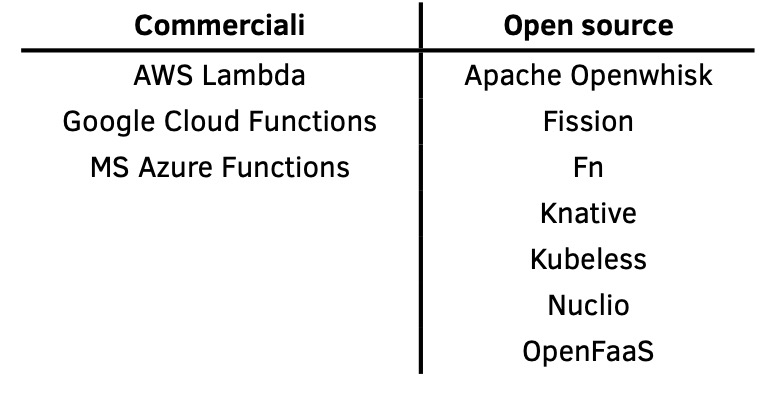
\includegraphics[width=0.5\textwidth]{13.png}
    \caption{FaaS commerciali vs Open Source}
    %\label{fig:enter-label}
\end{figure}

\paragraph{Business view}
\begin{itemize}
    \item Licensing: tutte le FaaS commerciali usano licenze proprietarie, a parte Azure che usa alcune open source. Tutte le FaaS open source usano Apache 2.0, quindi una licenza permissiva
    \item Installation: i server FaaS possono essere usati \textit{on-premise}, ovvero attraverso l’installazione, oppure \textit{as-a-service}, ovvero l’utilizzo del FaaS come servizio. Quasi tutte quelle open source sono disponibili on-premise mentre quelle commerciali sono as-a-service, tranne Azure che può essere installato
    \item Source code: le piattaforme commerciali non sono rilasciate come open source (ad eccezione di alcune parti di Azure). La scelta di un FaaS open source riduce i problemi di vendor lock-in
    \item Release: tutte le piattaforme commerciali sono sempre aggiornate e in produzione, mentre gli open source sono leggermente indietro rispetto alle piattaforme commerciali
    \item Interface: come l’operatore interagisce con il FaaS. Tutte le piattaforme supportano CLI, mentre API e le GUI non sono sempre fornite
    \item Community: GitHub è quello più utilizzato per gli open source. Su Stack Overflow c'è quasi tutto su AWS Lambda
    \item Documentation: tutte le piattaforme forniscono la documentazione su come sviluppare applicazioni e su come possiamo utilizzare la piattaforma. Per quanto riguarda lo sviluppo della piattaforma e dell’architettura, le piattaforme open source non forniscono molti dettagli
\end{itemize}


\paragraph{Technical view}
\begin{itemize}
    \item Development: i linguaggi di programmazione più supportati sono Java, Node.js, Python. Docker è sempre più supportato per poter personalizzare il runtime. La possibilità di usare degli editor o IDE è offerta dalla piattaforme commerciali
    \item Versioning: nel ciclo di vita di un progetto software ci sono più versioni della stessa applicazione. Questo è un punto di debolezza per le open source perché permettono spesso di fare solo implicit version. Le piattaforme commerciali permettono invece di avere dei meccanismi dedicati
    \item Event sources: tutte le piattaforme supportano l’invocazione sincrona basata su HTTP, mentre le invocazioni asincrone sono supportate da poche piattaforme. Molte piattaforme utilizzano schedulers per gestire il flusso di dati
    \item Function orchestration: nel codice ci possono essere più funzioni combinate tra loro. La maggioranza delle piattaforme offre un ”orchestratore” di funzioni dedicato, la metà delle piattaforme usano dei DSL specifici per i workflow, diagrammi di flusso, ...
    \item Testing e debugging: quasi tutte le piattaforme permettono di fare sia testing che debugging. Nelle piattaforme commerciali il testing e debugging sono integrate all’interno dell’ambiente. Nelle piattaforme open source si possono fare solo dei test call o debugging basato sui log
    \item Observability: per monitorare l’applicazione, gli strumenti sono forniti dal provider stesso in caso di piattaforme commerciali, mentre gli open source integrano servizi di terze parti.
    \item Application delivery: quasi tutte le piattaforme usano un approccio dichiarativo al deployment, cioè permettono all’utente di dichiarare qual è lo stato che vuole raggiungere, senza dover dichiarare i passi per raggiungerlo
    \item Code re-use: Lambda e Azure offrono tante funzioni built-in
    \item Access Management: per la gestione degli accessi, le piattaforme commerciali supportano autenticazione alle risorse mentre gli open source si appoggiano a servizi esterni
\end{itemize}
\newpage
\section{Laboratorio: AWS Lambda}

\paragraph{Spiegazione}
La funzione definita nel file (fornito su \href{https://elearning.di.unipi.it/enrol/index.php?id=334}{Moodle}) \verb|lambda_function.py| prende un file .txt all'interno di una cartella di un bucket S3 e ne crea una copia in una cartella \menu{crypted} sempre all'interno dello stesso bucket. Al contempo la cartella originale viene eliminata.\\
In un'ulteriore cartella \menu{decrypted} ne viene depositata una copia decifrata per verificare che il processo di cifratura sia andata a buon fine

\subsection{Procedimento}
\begin{enumerate}
    \item Creare \textbf{IAM role}:
    \begin{itemize}
        \item così come per EC2, anche per le Lambda Function dobbiamo prima concedere permessi per interagire con i bucket S3: la creazione di un IAM role per le lambda function è analoga al procedimento per EC2. Come caso d'uso scegliamo \textit{Lambda} e come policy scegliamo \textit{AmazonS3FullAccess}
    \end{itemize}

    \item Creare \textbf{bucket} S3:
    \begin{itemize}
        \item la nostra lambda function lavora interagendo con un bucket S3, quindi creiamo un bucket come abbiamo fatto nel primo laboratorio di AWS (si veda capitolo \ref{lab1}).
        Creiamo tre cartelle all'interno del Bucket: \menu{crypted/}, \menu{decrypted/}, \menu{plain/}
    \end{itemize}

    \item Creare la \textbf{Lambda function}:
    \begin{itemize}
        \item una volta pronti l'IAM role e il bucket S3, si procede con la creazione della lambda function.\\
        Settings: specificare \textit{creare da zero}, come runtime usare \verb|python3.8|, scegliere \textit{utliizza un ruolo esistente} e inserire il ruolo IAM creato prima.\\
        Dopo aver creato la lambda function, inserire il codice di \verb|lambda_function.py| \\
        Dopo qualsiasi modifica apportata apportata al codice, ricordarsi di clickare su \textbf{Deploy}
    \end{itemize}

    \item \textbf{Testare} la Lambda function:
    \begin{itemize}
        \item generare un evento di test selezionando come struttura quella di default
        \textbf{reminder}: le Lambda functions lavorano ricevendo in input e rispondendo in output oggetti JSON\\
        La nostra funzione restituisce il seguente errore:
        \begin{lstlisting}{json}
        {
        "errorMessage": "Unable to import module 'lambda_function': No module named 'cryptography'", 
        "errorType": "Runtime.ImportModuleError", 
        "stackTrace": []
        }
        \end{lstlisting}
    \end{itemize}

    \item Creare un livello in AWS Lambda:
    \begin{itemize}
        \item quando si crea una funzione in AWS Lambda bisogna specificare il Runtime da utilizzare, tuttavia il Runtime contiene solo librerie di base. Se si vogliono utilizzare altre librerie bisogna creare dei Livelli Lambda che verranno utilizzati dalle nostre funzioni
        Un \textbf{Livello Lambda} è un archivio di file .zip che può contenere codice o dati aggiuntivi e permette di impacchettare librerie e altre dipendenze da usare insieme alle lambda functions
        Nel nostro caso, la libreria \verb|cryptography| non fa parte del Runtime quindi dobbiamo inserirla tramite un livello: a tal fine creiamo un nuovo livello utilizzando l'archivio presente su \href{https://elearning.di.unipi.it/enrol/index.php?id=334}{Moodle} (\menu{python.zip}) che contiene già tutto il necessario
    \end{itemize}

    \item Aggiungere il livello:
    \begin{itemize}
        \item Dopo aver creato il livello, dobbiamo aggiungerlo alla nostra funzione cliccando su \textit{aggiungi un livello} $\rightarrow$ \textit{livelli personalizzati} $\rightarrow$ scegliere il livello appena creato e la versione di default.\\
        Adesso, riprovando ad eseguire il test, otteniamo un errore diverso:
        \begin{lstlisting}{json}
        { 
        "errorMessage": "'Records'",
        "errorType": "KeyError",
        "stackTrace": [ " File \"/var/task/lambda_function.py\", line 42, in lambda_handler\n for record in event['Records']:\n" ]
        }
        \end{lstlisting}
        questo errore indica che la funzione va in esecuzione ma l'input che riceve è mal formattato. Infatti, abbiamo usato un input di default e adesso dobbiamo creare un input che possa essere eseguito dalla funzione
    \end{itemize}

    \item Creare un livello in AWS Lambda:
    \begin{itemize}
        \item come evento possiamo usare il seguente, in cui sostituire \textit{BUCKET} con il nome del nostro bucket e, prevedibilmente, \textit{FILENAME} con il nome di un file .txt da cifrare, tra quelli precedentemente caricati nella cartella \menu{plain/} del nostro bucket
        \begin{lstlisting}{json}
            {
            "Records": [
              { "s3": { 
                        "bucket": { "name": "BUCKET" },
                        "object": { "key": "plain/FILENAME" } 
                        } 
              } ]
            }
        \end{lstlisting}
    \end{itemize}

    \item Aggiungere un \textbf{Trigger}:
    
    è possibile automatizzare l'esecuzione delle Lambda Functions in modo che vengano lanciate automaticamente ogni volta che si verifica un determinato evento.\\
    Nel nostro caso vogliamo che l'esecuzione della lambda function sia triggerata ogni volta che viene caricato un file nella cartella \menu{plain/} del bucket: per fare ciò, clickare su \textit{Aggiungi trigger} $\rightarrow$ scegliere S3 come origine e cliccare sul bucket di interesse $\rightarrow$ tipo di evento: \textit{tutti gli eventi di creazione oggetti} $\rightarrow$ aggiungere \textbf{.txt} come suffisso per far sì che la funzione venga chiamata solo quando il file caricato è un file testuale $\rightarrow$ accettare le condizioni sull'invocazione ricorsiva
    
\end{enumerate}

\subsection{Esercizi facoltativi (consigliati)}
\begin{enumerate}
    \item Test: verificare i casi limite o di errore, e.g. il file non è presente nel bucket o il bucket non è stato creato

    \item Analizzare il codice della funzione ed eliminare le parti di codice che eliminano il file originale dopo la cifratura

    \item Leggere la \href{https://docs.aws.amazon.com/it_it/lambda/latest/dg/services-apigateway- tutorial.html}{documentazione AWS su Lambda e API gateway} (link \href{https://docs.aws.amazon.com/it_it/lambda/latest/dg/services-apigateway- tutorial.html}{here})
\end{enumerate}
\newpage
\section{PaaS (Platform as a Service)}

\paragraph{\href{https://www.youtube.com/watch?v=6L1eQe5E1K4}{What is PaaS}} 
I PaaS aumentano i servizi offerti da IaaS, offrendo un intero ambiente di sviluppo e gestione dell’applicazione. I vantaggi del PaaS sono i seguenti:
\begin{itemize}
    \item \textit{"user just provides application and data"}
    \item Creare nuove versioni e farne il deployment più rapidamente
    \item Assemblare in modo semplice le varie parti dell’applicazione
    \item Scala automaticamente
    \item Non bisogna preoccuparsi della sicurezza
\end{itemize}

\begin{figure}[h!]
    \centering
    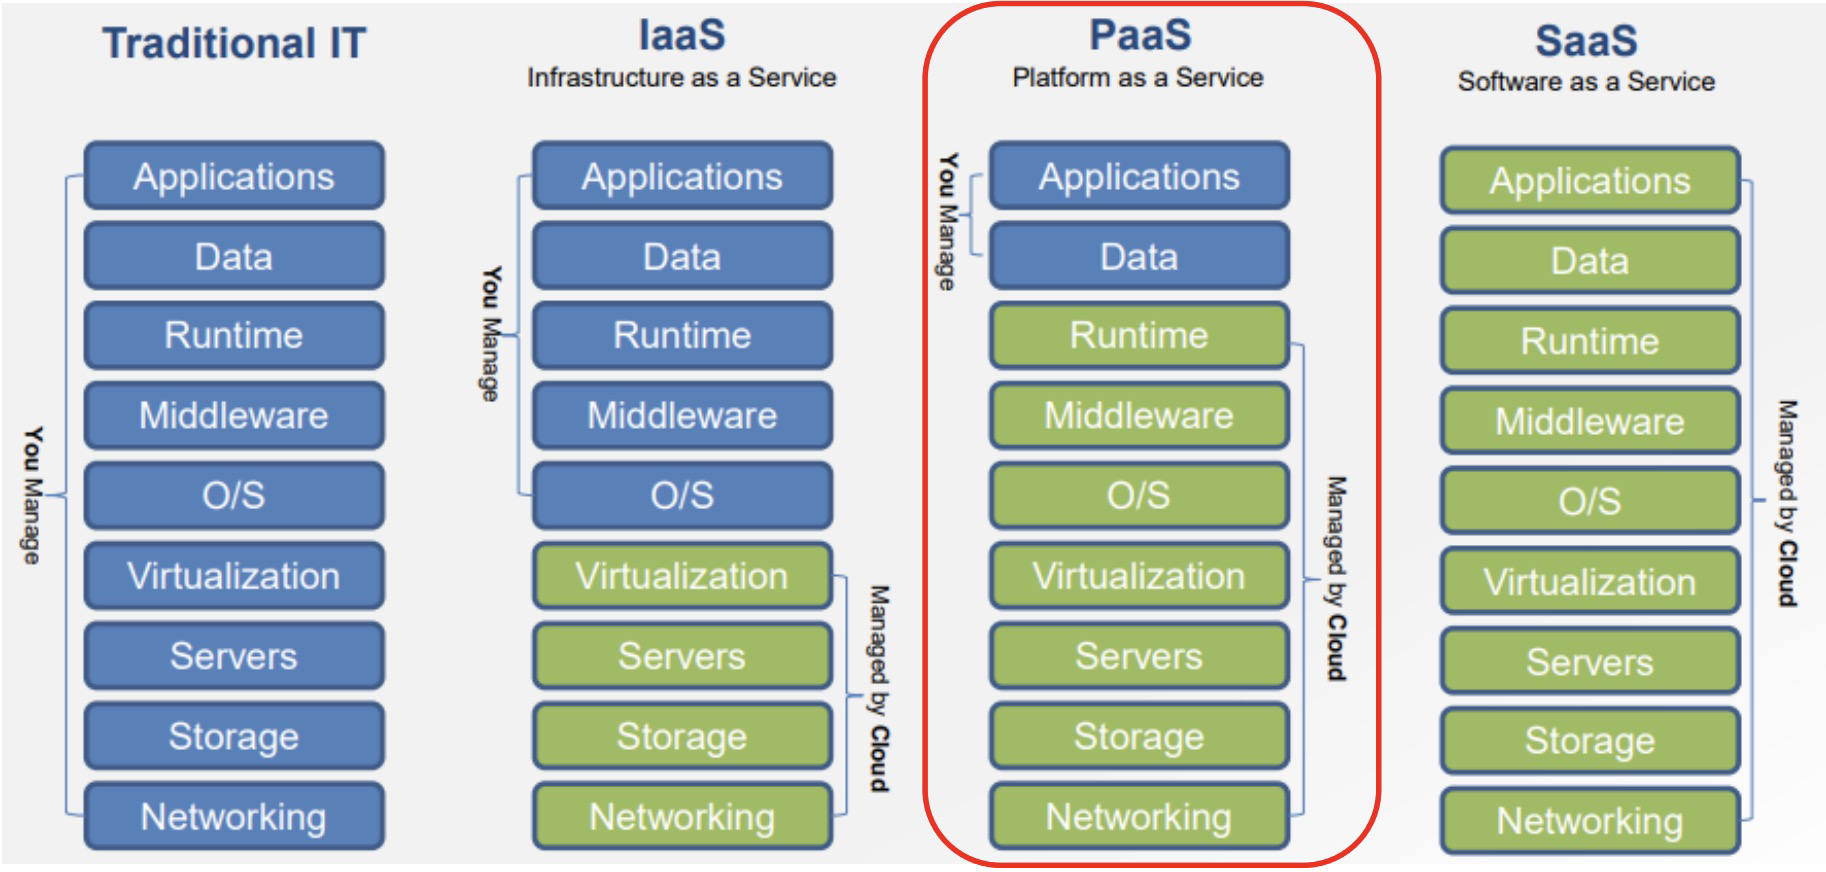
\includegraphics[width=0.7\textwidth]{14.png}
    \caption{Comparison: IaaS vs PaaS vs SaaS}
    % \label{fig:enter-label}
\end{figure}

\paragraph{Fetta di mercato} PaaS $<$ IaaS $<$ SaaS dovuto al fatto che l'utente target del PaaS è uno sviluppatore, mentre IaaS e SaaS sono rivolti ad un bacino di utenza molto più vasto.  Il PaaS attrae principalmente per l'aspetto di \textbf{application development}
\begin{figure}[h!]
    \centering
    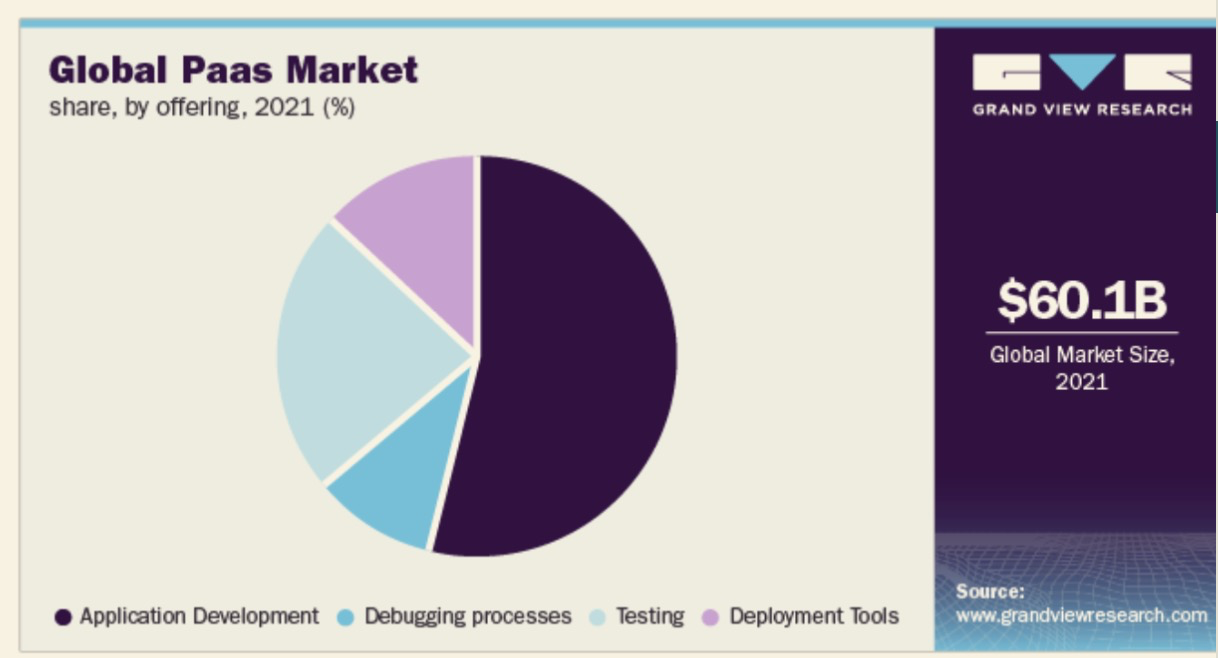
\includegraphics[width=0.7\textwidth]{15.png}
    \caption{Il servizio di PaaS più usato è quello di Application Development}
    % \label{fig:enter-label}
\end{figure}

\subsection{Heroku}
Heroku è una piattaforma Cloud che fornisce servizi integrati e un intero sistema che permette non solo di fare il deployment delle applicazioni, ma anche di modificarle, mandarle in esecuzione e gestirle.\\
Heroku nasce nel 2007 e viene acquisito da Salesforce nel 2010 per \$212M\\
I Container risolvono il grosso problema della \textbf{portabilità}: tramite Docker viene prelevata l’immagine del Container e ricostruita l’applicazione.  Heroku utilizza un sistema di Container chiamati \textbf{Dynos}, containers Linux virtualizzati che eseguono il codice fornito dall’utente: in pratica Heroku prende dall'utente un'applicazione non containerizzata e la incapscula in container.\\
I Dynos consentono una scalabilità molto flessibile, infatti a seconda delle richieste e delle risorse l’applicazione può scalare arbitrariamente il numero di Dynos.\\
Si può anche gestire il tipo, numero e dimensione di Dynos per applicazione, quindi l’utente non si deve preoccupare della gestione dell’infrastruttura e della scalabilità dell’applicazione.\\

\paragraph{Funzionamento} L'applicazione riceve la richiesta e la inoltra ad uno dei \textit{Web Dynos}; la richiesta viene analizzata e messa in coda asincrona (ottima per la scalabilità orizzontale); il \textit{Worker Dyno} gestisce la richiesta e la soddisfa, se è necessario può memorizzare in maniera persistente il risultato in un database. In questo caso la scalabilità permette di aumentare il numero di Web Dynos in modo da poter gestire un elevato numero di richieste contemporaneamente
\begin{figure}[h!]
    \centering
    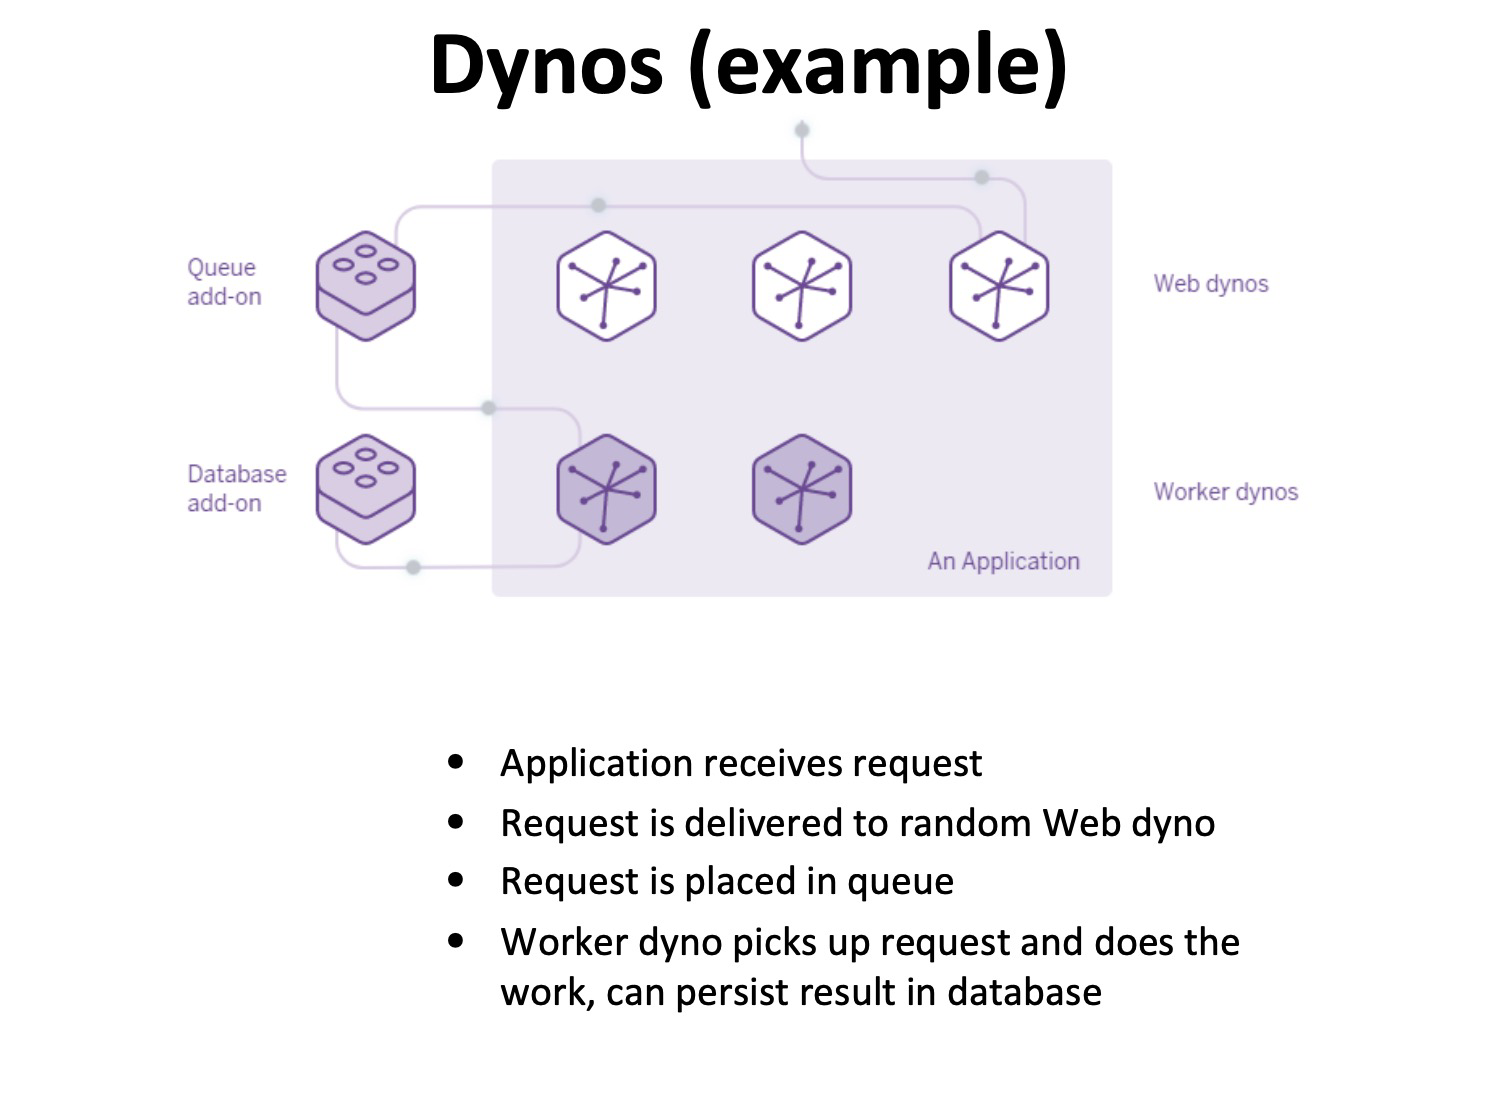
\includegraphics[width=0.7\textwidth]{16.png}
    \caption{Schema che rappresenta il funzionamento dei Dynos di Heroku}
    % \label{fig:enter-label}
\end{figure}

\subsubsection{Fasi Heroku}
\begin{enumerate}
    \item \textbf{Buildtime}: Heroku richiede tre componenti per costruire l'applicazione
    \begin{enumerate}
        \item codice sorgente
        \item lista di dipendenze
        \item un \textit{procfile},cioè un file di testo che contiene il comando per far partire il codice
    \end{enumerate}
    Una volta fornite queste tre cose, parte il sistema automatico di build: dopo aver ricevuto il codice, scarica il \textit{Build Packet} (linguaggio, dipendenze, librerie, ...), produce uno \textbf{slug} e lo mette in esecuzione in un Dynos. Il componente finale per eseguire l’applicazione è il sistema operativo (Ubuntu) che è aggiunto autonomamente da Heroku e si chiama \textbf{stack}

    \item \textbf{Runtime}: quando si fa il deployment o si scala manualmente l’applicazione, Heroku crea uno o più Dynos dove ognuno avrà lo stesso stack e slug che rappresenta un'istanza dell’applicazione.\\
    A questo punto Heroku esegue il comando che l’utente ha specificato nel \textit{procfile} per lanciare l’applicazione. Heroku permette di configurare le risorse che a tempo di esecuzione si vogliono utilizzare, per esempio esistono quattro tipi principali di Dynos:
    \begin{enumerate}
        \item \textit{free/hobby}, che comprendono le funzionalità di base
        \item \textit{standard}, che supportano la scalabilità orizzontale
        \item \textit{performance}, che oltre alla scalabilità orizzontale supporta anche l'\textbf{autoscaling} in cui si stabilisce a priori secondo quali parametri Heroku dovrà scalare
    \end{enumerate}

    \item \textbf{Add-ons}: Heroku ha 150+ add-ons che gli sviluppatori possono utilizzare per estendere le funzionalità dell’applicazione.\\
    Per esempio servizio di autenticazione, logging, monitoring, data stores... Tutto questo attrae l’utente perché può integrare rapidamente nuove features senza doverle costruire lui stesso from scratch.\\
    L’aspetto negativo è che l'utente è legato all’utilizzo della piattaforma e instaura una forma di \textbf{vendor lock-in} rendendo la nostra applicazione più difficilmente portabile. Infatti se volessimo spostare la nostra applicazione su un nuovo servizio Cloud saremo costretti a rivedere tutto il codice perché gli add-ons non sarebbero più disponibili
\end{enumerate}

\begin{figure}[h!]
    \centering
    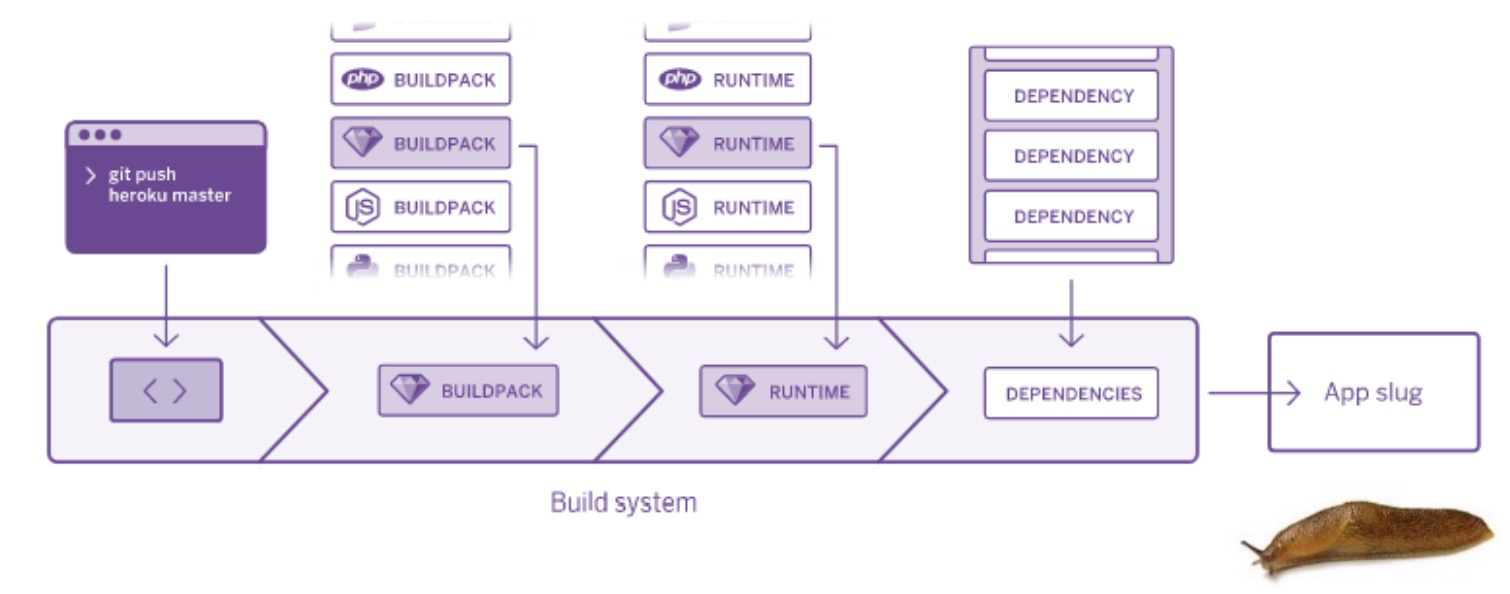
\includegraphics[width=0.7\textwidth]{17.png}
    \caption{Schema che rappresenta le fasi di Heroku per produrre l'app slug}
    % \label{fig:enter-label}
\end{figure}

\subsection{\href{https://www.youtube.com/watch?v=0d1OO79brYY}{Microsoft Azure}}
Microsoft Azure offre funzionalità simili a Heroku tra cui:
\begin{itemize}
    \item scalabilità verticale
    \item supporto di diversi linguaggi
    \item strumenti per sviluppatori (developer tools)
    \item SQL database
    \item meccanismi di sicurezza
    \item data storage
    \item machine learning per analisi predittive
    \item servizi media per supportare video.
\end{itemize}
Azure, che viene presentato come PaaS, è in realtà un \textit{IaaS+PaaS} perché la API che fornisce è molto ricca di funzionalità 

\subsection{\href{https://www.youtube.com/watch?v=XfTRyF6TX6o&list=PLaR6Rq6Z4Iqficb-XqeydZD_ZTD3XEwBp}{OpenShift}}
Red Hat OpenShift è una piattaforma PaaS molto utilizzata. Ci sono molte funzionalità semplici per il build e il deployment automatico. OpenShift è basato su Kubernetes (si veda capitolo \ref{container}) e può monitorare lo stato delle applicazioni facendole ripartire automaticamente in caso di fallimenti.\\
E` una piattaforma DevOps che permette la costruzione e l’erogazione dei servizi, infatti con OpenShift un'organizzazione può costruire il proprio workflow DevOps cioè un modo di lavorare che permette ai team di collaborare mantenendo autonomia.
\paragraph{Consigliato} \href{https://www.youtube.com/watch?v=IO_uap5wfUU}{OpenShift for Beginners - demo voting app}

\subsection{Google Firebase}
Firebase è il PaaS di Google, successore del primo PaaS che presentò (ai tempi chiamato \textit{GAE}). Il prossimo laboratorio sarà dedicato ad un \textit{hands-on} su Google Firebase. (si veda capitolo \ref{lab4})
%\newpage
\section{Laboratorio: Google Firebase} \label{lab4}

\paragraph{Obiettivo della lezione} Creazione di un evento RSVP per realizzare un invito interattivo, offrendo una chat per gli ospiti oltre ai dettagli dell'evento.\\
La caratteristica chiave dei PaaS è l'alto livello di astrazione garantito dalle estensioni (\textbf{add-ons}) che semplificano lo sviluppo dando l'opportunità di integrare funzionalità avanzate. 
Nella nostra applicazione integriamo l'auth tramite email:pass usando \textit{Firebase Authentication} e \textit{FirebaseUI}.
La chat è realizzata con \textit{Cloud Firestore} mentre la sicurezza per il database è garantita con \textit{Firebase Security rules}

\paragraph{\href{https://firebase.google.com/codelabs/firebase-get-to-know-web#0}{Tutorial creazione RSVP event}} durante tutto il procedimento abbiamo usato Stackblitz, un editor online in cui sono integrati workflows di Firebase. I file principali su cui lavoriamo sono \verb|index.js| e \verb|index.html|
\begin{enumerate}
    \item Come prima cosa creiamo un nuovo progetto Firebase:
    \begin{itemize}
        \item scegliere i metodi di autenticazione, noi abbiamo selezionato solo "Email/Password"
    \end{itemize}
    
    \item Creiamo un database, inizialmente in modalità "test", il che significa che il DB è aperto per letture e scritture. Più avanti nel codelab scriviamo le nostre regole di sicurezza custom made
    
    \item Al fine di utilizzare Firebase nell'app, importiamo varie librerie con degli \verb|import| statements in \verb|index.js|.\\
    E' fondamentale includere in \verb|index.js| anche il nostro oggetto di configurazione Firebase:
    \begin{lstlisting}[languague=Javascript]
    // Your web app's Firebase configuration
    const firebaseConfig = {
      apiKey: "your_api_key",
      authDomain: "labcloud-firebase.firebaseapp.com",
      projectId: "labcloud-firebase",
      storageBucket: "labcloud-firebase.appspot.com",
      messagingSenderId: "584194338624",
      appId: "1:584194338624:web:bc611483abd2b251c114a5",
      measurementId: "G-TY9GPL15Y6"
    };
    \end{lstlisting}

    \item Aggiungere accesso utente (\textbf{RSVP}): per aggiungere nuove features si deve
    \begin{enumerate}
        \item importare nuovi pacchetti dalle librerie
        \item modificare opportunamente \verb|index.html| (ad esempio aggiungere buttone per RSVP)
        \item aggiungere un \textbf{event listener} in \verb|index.js|
    \end{enumerate}
    
    \item Integrare la chat e archiviare tutti i messaggi inviati tramite \textbf{Cloud Firestore} (in pratica è un database NoSQL).  Ogni messaggio della chat viene archiviato come un documento dentro una raccolta chiamata \textit{guestbook} . Anche in questo caso occorre modificare l'html per includere un field nella pagina per scrivere i messaggi e un event listenere nel file js
    \begin{figure}[h!]
    \centering
    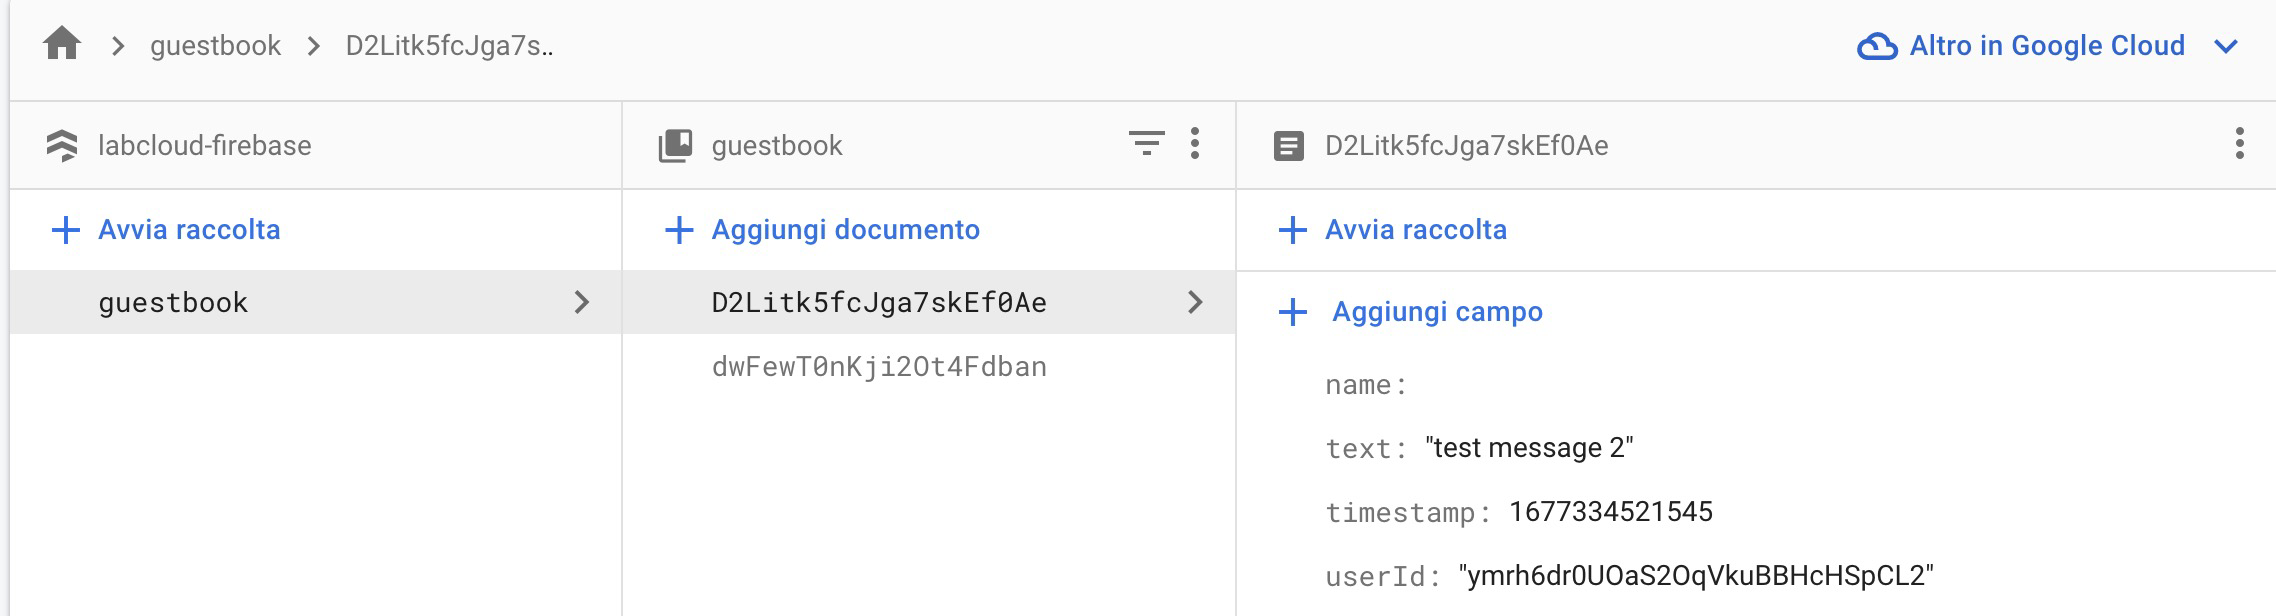
\includegraphics[width=0.7\textwidth]{18.png}
    \caption{Interfaccia che mostra i dettagli di ogni messaggio inviato nella chat}
    % \label{fig:enter-label}
\end{figure}

    \item Modifichiamo le \textbf{Rules} del DB:
    \begin{lstlisting}
    rules_version = '2';
    service cloud.firestore {
        match /databases/{database}/documents {
            match /guestbook/{entry} {
                allow read: if request.auth.uid != null;
                allow create:
                    if request.auth.uid == request.resource.data.userId;
            }
        }
    }
    \end{lstlisting}
    Per il libro degli ospiti solo gli utenti che hanno effettuato l'accesso possono leggere i messaggi (qualsiasi messaggio!), ma puoi creare un messaggio solo utilizzando il tuo ID utente.\\
    Inoltre, nel nostro esempio non consentiamo la modifica o l'eliminazione dei messaggi.

    \item Infine abbiamo aggiunto un bottone "\textit{Are you attending?}" per poter visualizzare quante persone hanno confermato la loro partecipazione
\end{enumerate}

\end{document}